\documentclass[12pt]{article}

% ============================================================
% 1. PAGE LAYOUT AND TYPOGRAPHY
% ============================================================

\usepackage[margin=2.5cm]{geometry} % Page margins
\usepackage{setspace}              % Line spacing options

% \doublespacing                   % Uncomment for double spacing

% Prevent overfull lines by allowing extra spacing flexibility
\setlength{\emergencystretch}{2em}

% Optional: Times-like text and matching mathematical fonts
\usepackage[T1]{fontenc}         % Improved font encoding

% ============================================================
% 2. MATHEMATICS AND SYMBOLS
% ============================================================

\usepackage{amsmath}   % Advanced mathematical environments
\usepackage{amssymb}   % Additional mathematical symbols
\usepackage{amsthm}    % Theorem and proof environments
\usepackage{bm}        % Bold mathematical symbols

% ============================================================
% 3. FIGURES, TABLES, AND FLOAT PLACEMENT
% ============================================================

\usepackage{graphicx}  % Insert and resize figures
\usepackage{booktabs}  % Professional-looking tables
\usepackage{float}     % Precise float placement, e.g., [H]
\usepackage{placeins}  % Restrict float movement using \FloatBarrier
\usepackage{rotating}  % Sideways figures and tables

% Default directory for figures
\graphicspath{{figures/}}

% Control the proportion of a page occupied by floats
\renewcommand{\topfraction}{0.9}       % Max. fraction for top floats
\renewcommand{\bottomfraction}{0.8}    % Max. fraction for bottom floats
\renewcommand{\textfraction}{0.1}      % Min. fraction reserved for text
\renewcommand{\floatpagefraction}{0.8} % Min. fraction on float-only pages


% ============================================================
% 4. CAPTION FORMATTING
% ============================================================

\usepackage{caption}              % Customize figure/table captions
\captionsetup{font=small}          % Set caption font size

% Display "Figure 1" and "Table 1" in bold
\makeatletter
\renewcommand{\fnum@figure}{\textbf{Figure \thefigure}}
\renewcommand{\fnum@table}{\textbf{Table \thetable}}
\makeatother


% ============================================================
% 5. REFERENCES, COLORS, AND HYPERLINKS
% ============================================================

\usepackage[authoryear]{natbib} % Author-year citations
\usepackage{xcolor}            % Custom colors
\usepackage{url}               % Format URLs
\usepackage{hyperref}          % Clickable links and references

% Define a custom blue for hyperlinks
\definecolor{mycustomblue}{HTML}{023C85}

% Hyperlink appearance
\hypersetup{
    colorlinks=true,
    linkcolor=mycustomblue, % Internal references
    citecolor=mycustomblue, % Bibliographic citations
    urlcolor=mycustomblue,  % External URLs
    filecolor=mycustomblue  % Local file links
}


% ============================================================
% 6. CUSTOM MATHEMATICAL NOTATION
% ============================================================

% Number sets and statistical operators
\newcommand{\R}{\mathbb{R}}       % Real numbers
\newcommand{\N}{\mathbb{N}}       % Natural numbers
\newcommand{\E}{\mathbb{E}}       % Expectation
\newcommand{\Var}{\mathbb{VAR}}   % Variance

% Upright mathematical symbols
\newcommand{\e}{{\rm e}}         % Euler's number
\newcommand{\dd}{{\rm d}}        % Differential


% ============================================================
% 7. THEOREM-LIKE ENVIRONMENTS
% ============================================================

\newtheorem{definition}{Definition}
\newtheorem{proposition}{Proposition}
\newtheorem{corollary}{Corollary}
\newtheorem{lemma}{Lemma}
\newtheorem{remark}{Remark}

% ============================================================
% END OF PREAMBLE
% ============================================================


% \title{Laguerre Weibull Distribution}
\title{A Gamma-Frailty Laguerre–Weibull Mortality Model with Actuarial Applications}

\author{
  \begin{tabular}[t]{c}
    {Fredy Castellares}\thanks{Corresponding author. \texttt{fredy.castellares@unifesp.br}; ORCID: \textcolor{red}{[to be added]}} \\
    \small{Universidade Federal de S\~ao Paulo} \\
    \small{S\~ao Paulo/SP, Brazil}
  \end{tabular}%
  \hspace*{2em}% Space between authors
  \begin{tabular}[t]{c}
    {Silvio C. Patricio}\thanks{\texttt{silca@sam.sdu.dk}; ORCID: 0000-0002-1025-5571} \\
    \small{University of Southern Denmark} \\
    \small{Odense, Denmark}
  \end{tabular}
}
\begin{document}
\maketitle

\vspace{-1cm}
\begin{abstract} \noindent
Annuity values depend on the shape of mortality at old ages. In the gamma-Gompertz model with positive frailty variance, the population hazard always levels off at old ages. We study the gamma--Laguerre--Weibull (GLW) model, which adds gamma frailty to the Laguerre--Weibull (LW) distribution and contains the gamma-Gompertz model as a special case. The LW distribution, a known Weibull extension, is derived from the generating function of the Laguerre polynomials, which gives a series representation in terms of distributions of maxima. The model includes a shape parameter $b$ that, for positive frailty variance, determines whether the population hazard grows without bound, levels off or declines at old ages. We derive moments, generating functions, entropy and Kullback--Leibler divergence, and life annuities, assurances and joint-life statuses. Parameters are estimated by maximum likelihood, and $b=1$ is tested by a likelihood-ratio test, bootstrap-calibrated when the frailty variance is estimated at zero. Simulations show small bias and correct test size. For female mortality at ages 50--109 in six countries, 1950--2020, $\hat b$ rises from about 1 to 1.23--1.37, the gamma-Gompertz restriction is rejected in every year from 1990, and the GLW model has the lowest AIC in 78\% of population-years among four models.\\
[0.5em]
\textbf{Keywords:} Laguerre polynomials; gamma frailty; gamma-Gompertz model; old-age mortality; life annuities; Poisson likelihood; likelihood-ratio test; Human Mortality Database.
\end{abstract}


%  ------------------------------------------------------------
\section{Introduction}
%  ------------------------------------------------------------

Parametric mortality laws have been used in actuarial work since \citet{gompertz1825} proposed that the force of mortality increases approximately exponentially with age. A law with few parameters smooths the observed death rates, and when its survival function is available in closed form, premiums, reserves and annuity values can be written as functions of the parameters. \citet{castellares2022gompertz, castellares2024gamma} derived such expressions for the Gompertz--Makeham and gamma-Gompertz--Makeham models.

At the oldest ages, the increase of observed mortality slows down and the hazard bends below the Gompertz curve \citep{vaupel1998biodemographic}, and insurers need reliable estimates of mortality at these ages to price life annuities \citep{gbari2017extreme}. Unobserved heterogeneity in frailty explains part of this pattern, because the frailest individuals die first and the population hazard therefore rises more slowly than the individual hazard \citep{vaupel1979impact}. With gamma frailty of mean one and variance $\sigma^2$, the population hazard is $\mu(x)/\{1+\sigma^2\int_0^x\mu(t)\,\dd t\}$, where $\mu$ is the individual hazard. Frailty thus produces the deceleration, but the form of $\mu$ determines whether the population hazard levels off, keeps rising or declines at old ages. For the Gompertz hazard $\mu(x)=\theta a\,\e^{ax}$ and $\sigma^2>0$, the population hazard always levels off at $a/\sigma^2$, so the gamma-Gompertz model cannot describe a hazard that keeps rising or declines. We propose a mortality model that keeps gamma frailty, adds a shape parameter to the individual hazard and contains the gamma-Gompertz model as a special case.

The model is built from the generating function of the Laguerre polynomials, which contains the factor $\exp\{-\theta t/(1-t)\}$. This factor has the form of the Gibbs weights $\exp(-\beta E)$ of statistical mechanics, with $\theta$ in the role of the inverse temperature $\beta$ and $t/(1-t)$ in that of the energy $E$ \citep[see][]{georgii2011gibbs}. Read as a survival function on $(0,1)$, it defines a one-parameter Laguerre distribution. Composing it with a baseline distribution function $G$ gives the survival function $\exp\{-\theta G/(1-G)\}$, whose hazard is the baseline hazard multiplied by $\theta/(1-G)$, a factor that increases with age. Its distribution function is a series in $G^k$, the distribution functions of maxima of $k$ independent copies from $G$, whose coefficients are differences of consecutive Laguerre polynomials (Proposition~\ref{prop:series}). This survival function is an exponential distribution applied to the odds $G/(1-G)$, so it belongs to the T-X class of \citet{alzaatreh2013new} and to the Weibull-G family of \citet{bourguignon2014weibull} with the Weibull shape fixed at one. With a Weibull baseline it is the Weibull extension of \citet{xie2002modified}, which generalises the model of \citet{chen2000new} and is studied further by \citet{tang2003statistical}. We call it the Laguerre--Weibull (LW) distribution. It contains the Gompertz distribution as a special case, and its hazard is increasing or bathtub-shaped, depending on a shape parameter $b$. Adding gamma frailty gives the gamma--Laguerre--Weibull (GLW) model, which contains the gamma-Gompertz model as a special case. For positive frailty variance, $b$ determines whether the population hazard grows without bound, levels off or declines at old ages.

Since $\sigma^2\theta\{\exp(aX^b)-1\}$ follows a Pareto type II distribution, we derive the moments, the generating functions, the Shannon entropy and the Kullback--Leibler divergence of the GLW model in terms of special functions and series. For the actuarial calculations, we show that, if $T_x$ is the future lifetime at age $x$, then $a(x+T_x)^b-ax^b$ has the distribution of $aX^b$ with $\theta$ replaced by an age-dependent parameter $\theta_x$. When $b=1$ the future lifetime is therefore again gamma-Gompertz, and under a restriction on the parameters the joint-life status of two lives of the same age is again a GLW model. Life annuities and assurances are in general one-dimensional integrals, which we evaluate numerically.

The parameters are estimated by maximum likelihood from death counts and exposures to risk, with the death counts modelled as Poisson variables \citep{brillinger1986biometrics, macdonald2018modelling}, and the gamma-Gompertz model is tested against the GLW model with a likelihood-ratio test. We assess both in a simulation study. We then fit the model to female mortality after age 50 in six countries from 1950 to 2020, using the Human Mortality Database \citep{hmd}, compare it with the Gompertz, Kannisto and gamma-Gompertz models, and compute remaining life expectancies, annuities and assurances at ages 50, 65 and 80.

The contribution of the paper is the mortality model built on the LW distribution, together with the Laguerre representation, the analytical and actuarial properties of the model, likelihood inference with a test of the gamma-Gompertz restriction, and the application to seventy years of mortality data. Section~\ref{sec:laguerre} introduces the Laguerre distribution. Section~\ref{sec:family} defines the Laguerre-G family and the LW distribution. Section~\ref{sec:glw} presents the GLW model, and Section~\ref{sec:actuarial} its actuarial properties. Section~\ref{sec:inference} treats statistical inference, Section~\ref{sec:simulation} reports a simulation study, Section~\ref{sec:application} presents the application, and Section~\ref{sec:conclusion} concludes.


%  ------------------------------------------------------------
\section{The Laguerre distribution}\label{sec:laguerre}
%  ------------------------------------------------------------

The generating function of the Laguerre polynomials, given in Equation~\eqref{exp} below, contains the factor $\exp\{-\theta x/(1-x)\}$. A function $\exp\{-\theta\,g(x)\}$ with $g$ increasing from 0 to infinity is a survival function with cumulative hazard $\theta g$, and it has the exponential form of the Gibbs weights of statistical mechanics \citep[see][]{georgii2011gibbs}. With $g(x)=x/(1-x)$ on $(0,1)$, this survival function can be expanded in terms of Laguerre polynomials, as in Equation~\eqref{family}. The expansion gives the representations of this section and of Section~\ref{sec:family}, where the survival function is composed with a baseline distribution, which multiplies the baseline hazard by a factor that increases with age.

\subsection{Laguerre polynomials}

The Laguerre polynomials are
\begin{equation}\label{def-Lag}
L_n(\theta) = \sum_{k=0}^{n} \binom{n}{k}\, \frac{(-1)^k\,\theta^k}{k!}, \qquad n\in\N=\{0,1,2,\dots\}.
\end{equation}
More generally, the associated Laguerre polynomials $L_n^{(\alpha)}$, $\alpha>-1$, have generating function
\begin{equation}\label{exp}
\sum_{n=0}^{\infty} L_n^{(\alpha)}(\theta)\, x^n = \frac{1}{(1-x)^{\alpha+1}}\,\exp\left\{-\frac{\theta x}{1-x}\right\}, \qquad |x|<1,
\end{equation}
with $L_n=L_n^{(0)}$ \citep[see][]{lebedev1965special, rainville1960special}. For $\theta\geq 0$, $|L_n(\theta)|\leq \e^{\theta/2}$ for all $n$ \citep{szeg1939orthogonal}. Setting $\alpha=0$ in Equation~\eqref{exp} gives
\begin{equation}\label{family}
\exp\left\{-\frac{\theta x}{1-x}\right\}=(1-x)\sum^{\infty}_{n=0} L_{n}(\theta) \, x^n, \qquad |x|<1.
\end{equation}

\subsection{Definition and properties}

For $\theta>0$, the function $\phi(x)=\exp\{-\theta x/(1-x)\}$ is continuous and strictly decreasing on $(0,1)$, and it goes from 1 at $x=0$ to 0 as $x\to1$. It is therefore a survival function on $(0,1)$.

\begin{definition}
A random variable $X$ has the Laguerre distribution with parameter $\theta>0$, written $X\sim\mathcal{L}(\theta)$, if its distribution function is
\[
H(x)=1-\exp\left\{-\frac{\theta x}{1-x}\right\}, \qquad 0<x<1.
\]
\end{definition}

\begin{proposition}\label{prop:basic}
Let $X\sim\mathcal{L}(\theta)$.
\begin{enumerate}\renewcommand{\labelenumi}{(\roman{enumi})}
\item $T=X/(1-X)$ is exponentially distributed with rate $\theta$; equivalently, $X=T/(1+T)$.
\item The quantile function is $H^{-1}(u)=-\log(1-u)/\{\theta-\log(1-u)\}$, $0<u<1$.
\item The density and the hazard function are
\[
h(x)= \frac{\theta}{(1-x)^2}\, \exp\left\{-\frac{\theta x}{1-x}\right\},
\qquad
\nu(x)= \frac{\theta}{(1-x)^2}, \qquad 0<x<1.
\]
The hazard increases from $\theta$ to infinity.
\item For $0<x<1$,
\[
H(x)=x-\sum^{\infty}_{k=1} L_{k}(\theta) \, (x^k-x^{k+1}),
\qquad
h(x)=\theta\sum_{k=0}^{\infty} L_k^{(1)}(\theta)\, x^k.
\]
\end{enumerate}
\end{proposition}

\begin{proof}
(i) For $t>0$, the event $\{T>t\}$ is the event $\{X>t/(1+t)\}$. Hence $\Pr(T>t)=1-H\{t/(1+t)\}=\e^{-\theta t}$.

(ii) Setting $H(x)=u$ gives $\theta x/(1-x)=-\log(1-u)$, and solving for $x$ gives $H^{-1}(u)$.

(iii) Differentiating $H$ gives $h(x)=\theta(1-x)^{-2}\phi(x)$, because $\dd\{x/(1-x)\}/\dd x=(1-x)^{-2}$. The hazard is $\nu(x)=h(x)/\{1-H(x)\}=h(x)/\phi(x)=\theta(1-x)^{-2}$, which increases from $\theta$ at $x=0$ to infinity as $x\to1$.

(iv) By Equation~\eqref{family}, $1-H(x)=(1-x)\sum_{k\geq0}L_k(\theta)x^k=\sum_{k\geq0}L_k(\theta)(x^k-x^{k+1})$. Since $L_0=1$, the term with $k=0$ is $1-x$, and the expansion of $H$ follows. For $h$, Equation~\eqref{exp} with $\alpha=1$ gives $(1-x)^{-2}\phi(x)=\sum_{k\geq0}L_k^{(1)}(\theta)x^k$; multiplying by $\theta$ gives $h(x)$ by part (iii).
\end{proof}

Part (i) gives a simple way to simulate $X$: draw $T$ from an exponential distribution with rate $\theta$ and set $X=T/(1+T)$.

\begin{proposition}\label{prop:moments}
Let $X\sim\mathcal{L}(\theta)$, let $E_1(z)=\int_z^\infty t^{-1}\e^{-t}\,\dd t$ be the exponential integral, and let $q(\theta)=\theta\,\e^{\theta}E_1(\theta)$. For $n\geq 1$,
\begin{equation}\label{eq:moments}
\E[X^n]= n \sum_{k=0}^{\infty} \frac{L_k(\theta)}{(k+n)(k+n+1)}.
\end{equation}
The first two moments and the variance also have the closed forms
\[
\E[X]=1-q(\theta), \qquad \E[X^2]=1+\theta-(2+\theta)\,q(\theta), \qquad \Var[X]=\theta\{1-q(\theta)\}-q(\theta)^2.
\]
\end{proposition}

Equating the two expressions for $\E[X]$ gives a series for the exponential integral,
\begin{equation}\label{eq:E1}
E_1(\theta)=\frac{\e^{-\theta}}{\theta}\left\{\frac12 - \sum_{k=1}^{\infty} \frac{L_k(\theta)}{(k+1)(k+2)}\right\}, \qquad \theta>0.
\end{equation}


\begin{proof}
For a random variable on $(0,1)$, $\E[X^n]=\int_0^1 n x^{n-1}\Pr(X>x)\,\dd x$. With $\Pr(X>x)=(1-x)\sum_{k\geq0}L_k(\theta)x^k$ from Equation~\eqref{family},
\[
\E[X^n]=n\sum_{k=0}^{\infty}L_k(\theta)\int_0^1 x^{n+k-1}(1-x)\,\dd x=n\sum_{k=0}^{\infty}\frac{L_k(\theta)}{(k+n)(k+n+1)},
\]
which is Equation~\eqref{eq:moments}. Integrating term by term is justified because $|L_k(\theta)|\leq\e^{\theta/2}$ and $\sum_k\{(k+n)(k+n+1)\}^{-1}<\infty$.

For the closed forms, write $X=1-(1+T)^{-1}$, with $T$ exponential with rate $\theta$ (Proposition~\ref{prop:basic}(i)). By the definition of $E_1$,
\[
\E\left[(1+T)^{-1}\right]=\theta\int_0^\infty\frac{\e^{-\theta t}}{1+t}\,\dd t=\theta\,\e^{\theta}E_1(\theta)=q(\theta).
\]
Integrating by parts,
\[
\E\left[(1+T)^{-2}\right]=\theta\int_0^\infty\frac{\e^{-\theta t}}{(1+t)^2}\,\dd t=\theta\left\{1-\theta\int_0^\infty\frac{\e^{-\theta t}}{1+t}\,\dd t\right\}=\theta\{1-q(\theta)\}.
\]
Hence $\E[X]=1-q(\theta)$ and $\E[X^2]=1-2\E[(1+T)^{-1}]+\E[(1+T)^{-2}]=1+\theta-(2+\theta)q(\theta)$. The variance is $\E[X^2]-\E[X]^2$.
\end{proof}

\subsection{Estimation}

Given a sample $x_1,\dots,x_N$ from $\mathcal{L}(\theta)$, the maximum likelihood estimator of $\theta$ is
\[
\hat{\theta}=\frac{N}{\sum_{i=1}^{N} x_i/(1-x_i)},
\]
which is the usual estimator of an exponential rate applied to $t_i=x_i/(1-x_i)$. Its asymptotic variance is $\theta^2/N$.


%  ------------------------------------------------------------
\section{The Laguerre-G family and the Laguerre--Weibull distribution}\label{sec:family}
%  ------------------------------------------------------------

To obtain lifetime distributions, we transform the Laguerre distribution through a baseline distribution function.

\subsection{Definition}

Let $X\sim\mathcal{L}(\theta)$, and let $G$ be a continuous distribution function with density $g$, hazard $\mu_G=g/(1-G)$ and quantile function $G^{-1}$. We define the Laguerre-G random variable $Y=G^{-1}(X)$.

\begin{proposition}\label{prop:family}
The distribution function and the hazard function of $Y$ are
\[
F(x)=1- \exp\left\{-\theta\,\frac{G(x)}{1-G(x)}\right\},
\qquad
\mu_F(x)=\frac{\theta}{1-G(x)}\,\mu_G(x).
\]
\end{proposition}

\begin{proof}
Since $G$ is continuous and increasing, $\{Y\leq x\}=\{X\leq G(x)\}$, so $F(x)=H\{G(x)\}$, which gives the expression for $F$. The hazard of $Y$ is $\mu_F(x)=-\dd\log\{1-F(x)\}/\dd x=\theta\,\dd\{G(x)/(1-G(x))\}/\dd x=\theta\,g(x)/\{1-G(x)\}^2$, which equals $\theta\mu_G(x)/\{1-G(x)\}$.
\end{proof}

The ratio $\mu_F/\mu_G=\theta/(1-G)$ increases with $x$, from $\theta$ to infinity. Hence $\mu_F$ exceeds $\mu_G$ at every $x$ when $\theta\geq 1$. When $\theta<1$, it does so beyond the point where $G(x)=1-\theta$.

\begin{remark}
$F$ is an exponential distribution applied to the odds $G/(1-G)$. It belongs to the T-X class of \citet{alzaatreh2013new}, and it is the Weibull-G family of \citet{bourguignon2014weibull} with the Weibull shape parameter fixed at one.
\end{remark}

The Laguerre construction gives the following representation.

\begin{proposition}\label{prop:series}
Let $w_k(\theta)=L_{k-1}(\theta)-L_k(\theta)$ for $k\geq1$. Then $w_k(\theta)=(\theta/k)\,L_{k-1}^{(1)}(\theta)$, and for every $x$ with $G(x)<1$,
\[
F(x)=\sum_{k=1}^{\infty} w_k(\theta)\, G(x)^k,
\qquad
f(x)=\theta\, g(x)\sum_{k=0}^{\infty} L_k^{(1)}(\theta)\, G(x)^k.
\]
\end{proposition}

\begin{proof}
By Proposition~\ref{prop:family} and Equation~\eqref{family}, with $G=G(x)$,
\[
1-F(x)=(1-G)\sum_{n=0}^{\infty}L_n(\theta)G^n=L_0(\theta)+\sum_{k=1}^{\infty}\{L_k(\theta)-L_{k-1}(\theta)\}G^k.
\]
Since $L_0=1$, this gives $F(x)=\sum_{k\geq1}w_k(\theta)G^k$. The series for $f$ follows from $f(x)=g(x)\,h\{G(x)\}$ and Proposition~\ref{prop:basic}(iv). Both are power series in $G$ with radius of convergence one, so the series for $F$ can be differentiated term by term. This gives $f(x)=g(x)\sum_{k\geq1}k\,w_k(\theta)G^{k-1}$, and comparing coefficients with the series for $f$ gives $k\,w_k(\theta)=\theta L_{k-1}^{(1)}(\theta)$.
\end{proof}

Since $G^k$ is the distribution function of the maximum of $k$ independent copies from $G$, Proposition~\ref{prop:series} writes $F$ as a linear combination of distributions of maxima. Some weights $w_k(\theta)$ can be negative, so $F$ is not in general a mixture. Expectations under $F$ can still be computed term by term from those of the maxima. For example, $\E[Y^r]=\sum_k w_k(\theta)\,\E[M_k^r]$, where $M_k$ is the maximum of $k$ copies, whenever the series converges.

\subsection{Exponential baseline}

If $G(x)=1-\e^{-\lambda x}$, then $G/(1-G)=\e^{\lambda x}-1$, and
\[
F(x)=1-\exp\{-\theta(\e^{\lambda x}-1)\},\qquad \mu_F(x)=\theta\lambda\,\e^{\lambda x},\qquad x>0.
\]
$Y$ therefore follows the Gompertz law with initial level $\theta\lambda$ and rate $\lambda$.

\subsection{Weibull baseline}

If $G(x)=1-\exp(-ax^b)$, with $a,b>0$, then $G/(1-G)=\e^{ax^b}-1$, and
\begin{equation}\label{L-weibull}
F(x)=1- \exp\left\{-\theta\left(\e^{ax^b}-1\right)\right\},
\qquad
\mu_F(x)=\theta\,ab\,x^{b-1}\,\e^{ax^b}, \qquad x>0.
\end{equation}
We call this the Laguerre--Weibull (LW) distribution. With $\theta=\lambda\alpha$, $a=\alpha^{-\beta}$ and $b=\beta$, it is the Weibull extension of \citet{xie2002modified}, whose distribution function is $1-\exp[\lambda\alpha\{1-\e^{(x/\alpha)^\beta}\}]$. The model of \citet{chen2000new} is the case $a=1$.

\subsection{Shape of the LW hazard}

The parameter $\theta$ multiplies the hazard at every age. It sets the level of mortality and leaves its age pattern unchanged. The parameters $a$ and $b$ set the age pattern, and $a^{-1/b}$ acts as a scale for age, since $ax^b=(x/a^{-1/b})^b$. From
\[
\frac{\dd}{\dd x}\log\mu_F(x)=\frac{b-1}{x}+ab\,x^{b-1},
\]
the hazard is increasing when $b\geq1$. When $b=1$ it is the Gompertz hazard $\theta a\,\e^{ax}$, which grows at the constant relative rate $a$. When $b>1$ the relative rate of increase grows without bound at older ages, and mortality eventually rises faster than exponentially. When $0<b<1$ the hazard is bathtub-shaped. It decreases from infinity at $x=0$ to a minimum at $x^\ast=\{(1-b)/(ab)\}^{1/b}$ and increases afterwards \citep{xie2002modified}.

Figure~\ref{fig:lw} shows the density, survival function and hazard function of the LW distribution for four parameter sets, with the hazard on a log scale. The set with $b<1$ has a bathtub-shaped hazard. The set with $b=1$ has a Gompertz hazard, which is a straight line on the log scale. The two sets with $b>1$ have hazards that rise faster than exponentially.

\begin{figure}[htb!]
\centering
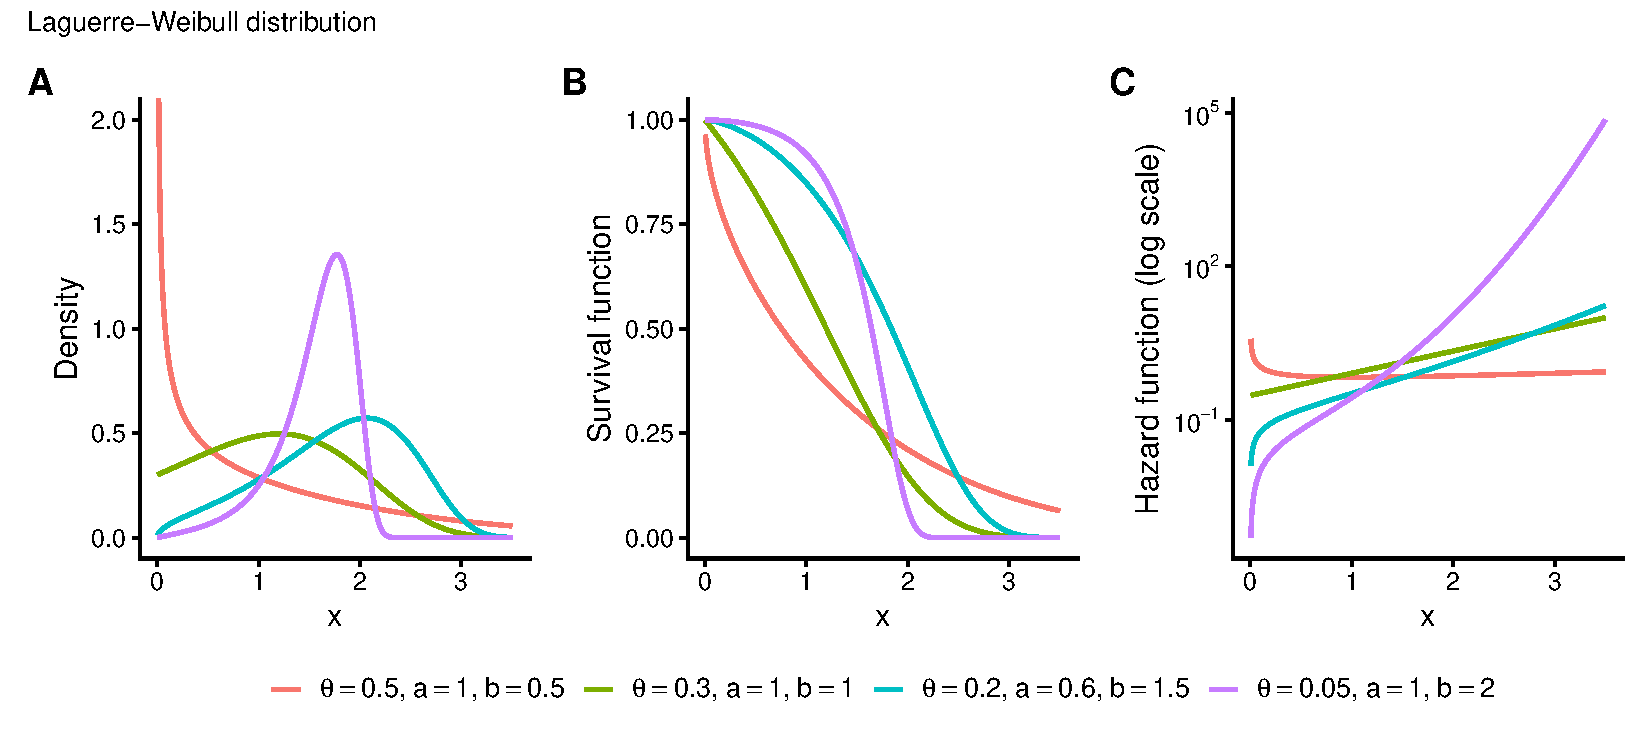
\includegraphics[width=\textwidth]{laguerre_weibull.pdf}
\caption{Laguerre--Weibull distribution for four parameter sets: (A) density, (B) survival function and (C) hazard function, on a log scale.}
\label{fig:lw}
\end{figure}


%  ------------------------------------------------------------
\section{The gamma--Laguerre--Weibull model}\label{sec:glw}
%  ------------------------------------------------------------

The LW hazard describes a homogeneous population. At old ages, the selective survival of the more robust makes the population hazard rise more slowly than individual hazards, so a mortality model needs to allow for unobserved heterogeneity. To this end, we multiply the LW hazard by an unobserved frailty $Z$, so that $\mu(x\mid Z=z)=z\,\mu_F(x)$, where $Z$ follows a gamma distribution with $\E[Z]=1$ and $\Var[Z]=\sigma^2$ \citep{vaupel1979impact}. Integrating over $Z$ gives the population survival function $S(x)=\{1+\sigma^2 M_F(x)\}^{-1/\sigma^2}$, where $M_F(x)=\theta(\e^{ax^b}-1)$ is the cumulative LW hazard. Throughout, we write $\rho=\sigma^2\theta$.

\subsection{Basic functions}

\begin{proposition}\label{prop:glw}
Under the gamma--Laguerre--Weibull (GLW) model, the survival function and the hazard function are, for $x>0$,
\begin{equation}\label{L-weibull-frailty}
S(x)=\left\{1+\rho\left(\e^{ax^b}-1\right)\right\}^{-1/\sigma^2}
\qquad\text{and}\qquad
\bar{\mu}(x) = \frac{\theta\, a b\, x^{b - 1}\, \e^{a x^{b}}}{1 + \rho \left(\e^{a x^{b}} - 1\right)}.
\end{equation}
\end{proposition}

\begin{proof}
Given $Z=z$, the survival function is $\exp\{-zM_F(x)\}$, so $S(x)=\E[\exp\{-ZM_F(x)\}]$. This is the Laplace transform of $Z$ evaluated at $M_F(x)$. For a gamma distribution with mean 1 and variance $\sigma^2$, $\E[\e^{-sZ}]=(1+\sigma^2s)^{-1/\sigma^2}$, which gives $S(x)$. The hazard is $\bar\mu(x)=-\dd\log S(x)/\dd x$.
\end{proof}

The GLW model reduces to the LW distribution as $\sigma^2\to0$, and to the gamma-Gompertz model when $b=1$. Every result below is stated for the GLW model, and the corresponding LW result follows by letting $\sigma^2\to0$.

\subsection{Shape of the GLW hazard}

From Equation~\eqref{L-weibull-frailty},
\[
\frac{\dd}{\dd x}\log\bar\mu(x)=\frac{b-1}{x}+ab\,x^{b-1}\,\frac{1-\rho}{1+\rho\left(\e^{ax^b}-1\right)}.
\]
Compared with the LW hazard, frailty multiplies the second term by a factor that equals $1-\rho$ at $x=0$ and decreases to zero as $x\to\infty$. We consider $\rho<1$, the relevant case for human mortality. As $x\to0$, $\bar\mu(x)$ behaves like the LW hazard $\theta ab\,x^{b-1}$, so it tends to zero when $b>1$, to $\theta a$ when $b=1$, and to infinity when $0<b<1$. When $\sigma^2>0$ and $x\to\infty$, $\bar\mu(x)$ behaves like $ab\,x^{b-1}/\sigma^2$. When $b=1$ the hazard increases and levels off at $a/\sigma^2$, as in the gamma-Gompertz model. When $b>1$ it increases without bound, but its relative rate of increase tends to zero, so it grows only polynomially at older ages. When $0<b<1$ it decreases near $x=0$ and declines to zero at older ages, possibly after rising over an intermediate range. When $\sigma^2=0$, $\bar\mu$ is the LW hazard, which grows without bound for every $b>0$ because of the factor $\e^{ax^b}$. Because $b$ is estimated mainly from ages with many deaths, the hazard implied at the oldest ages is an extrapolation.

Figure~\ref{fig:glw} shows the density, survival function and hazard function of the GLW model for four parameter sets, with the hazard on a log scale. The two sets with $b=1$ level off at $a/\sigma^2$, which equals 2 for $\sigma^2=0.5$ and 0.5 for $\sigma^2=2$. The set with $b<1$ declines towards zero after its initial decrease. The set with $b>1$ keeps increasing, although slowly, since $\bar\mu(x)$ behaves like $ab\,x^{b-1}/\sigma^2$.

\begin{figure}[htb!]
\centering
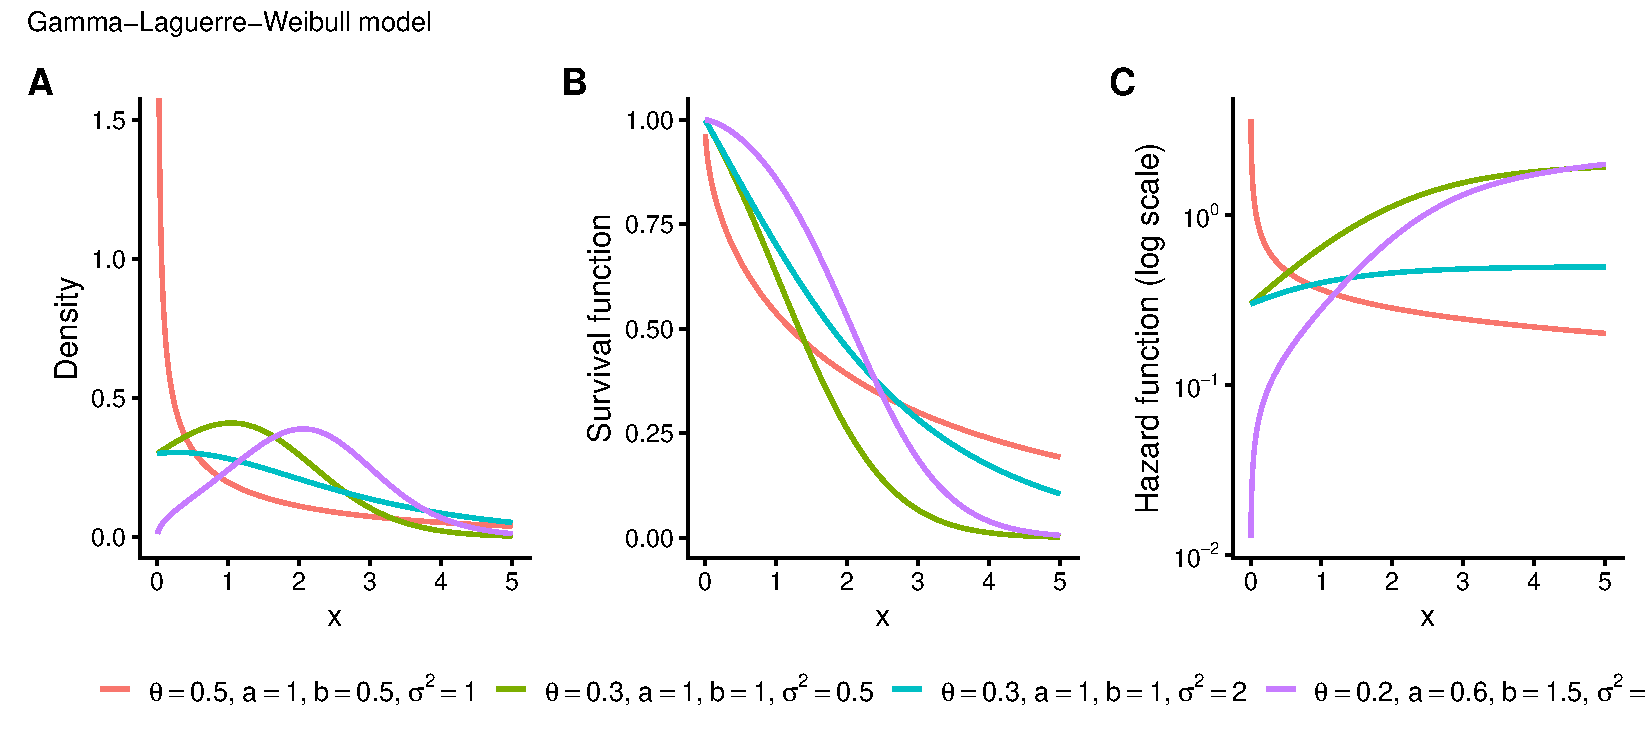
\includegraphics[width=\textwidth]{gamma_laguerre_weibull.pdf}
\caption{Gamma--Laguerre--Weibull model for four parameter sets: (A) density, (B) survival function and (C) hazard function, on a log scale.}
\label{fig:glw}
\end{figure}

\subsection{Stochastic representation}

The remaining subsections characterise the distribution of a GLW lifetime. Besides describing the statistical structure of the model, some of these results are used later: the moments give the remaining life expectancy at the starting age (Corollary~\ref{cor:ex}), the Laplace transform gives the annuity and assurance values there (Section~\ref{sec:actuarial}), and the representation below underlies the future-lifetime result of Proposition~\ref{prop:future}. Most of the results follow from a simple representation of $U=aX^b$.

\begin{proposition}\label{prop:repr}
Let $X$ follow the GLW model and let $V=\rho\,(\e^{aX^b}-1)$. Then $\Pr(V>v)=(1+v)^{-1/\sigma^2}$ for $v>0$, so that $V$ has a Pareto type II (Lomax) distribution with shape $1/\sigma^2$ and unit scale, and
\[
X=\left\{\frac1a\log\left(1+\frac{V}{\rho}\right)\right\}^{1/b}.
\]
Under the LW model, $\theta(\e^{aX^b}-1)$ is exponentially distributed with unit mean, and $X=[a^{-1}\log\{1+\mathcal{E}/\theta\}]^{1/b}$ with $\mathcal{E}$ a standard exponential random variable.
\end{proposition}

\begin{proof}
For $v>0$, $V>v$ if and only if $X>x_v$, where $x_v=\{a^{-1}\log(1+v/\rho)\}^{1/b}$. Since $1+\rho(\e^{ax_v^b}-1)=1+v$, Proposition~\ref{prop:glw} gives $\Pr(V>v)=S(x_v)=(1+v)^{-1/\sigma^2}$. Solving $V=\rho(\e^{aX^b}-1)$ for $X$ gives the representation. Under the LW model, $S(x)=\exp\{-\theta(\e^{ax^b}-1)\}$, and the same argument gives $\Pr\{\theta(\e^{aX^b}-1)>v\}=\e^{-v}$.
\end{proof}

\subsection{Moments}

The moments involve two special functions. The first is the generalised Hurwitz--Lerch zeta function of \citet{goyal1997generalized},
\[
\Phi^\ast_\mu(z,s,v)=\sum_{n=0}^{\infty}\frac{(\mu)_n}{n!}\,\frac{z^n}{(n+v)^s}
=\frac{1}{\Gamma(s)}\int_0^\infty t^{s-1}\e^{-vt}\left(1-z\e^{-t}\right)^{-\mu}\dd t,
\]
where $(\mu)_n=\Gamma(\mu+n)/\Gamma(\mu)$. The series converges for $|z|<1$, and the integral defines $\Phi^\ast_\mu$ for every $z<1$ when $s,v>0$. The second is the generalised integro-exponential function of \citet{milgram1985generalized},
\[
E_s^j(z)=\frac{1}{\Gamma(j+1)}\int_1^\infty(\log t)^j\,t^{-s}\,\e^{-zt}\,\dd t,
\]
which reduces to the exponential integral $E_1(z)$ when $s=1$ and $j=0$.

\begin{proposition}\label{prop:moments-glw}
Under the GLW model, for $r>0$,
\begin{equation}\label{eq:glw-moments}
\E[X^r]=\frac{\Gamma(r/b+1)}{\sigma^2\,a^{r/b}\,\rho^{1/\sigma^2}}\;\Phi^\ast_{1+1/\sigma^2}\!\left(1-\frac1\rho,\;\frac rb+1,\;\frac1{\sigma^2}\right).
\end{equation}
Under the LW model,
\begin{equation}\label{eq:lw-moments}
\E[X^r]=\theta\,\e^{\theta}\,\Gamma(r/b+1)\,a^{-r/b}\,E_0^{r/b}(\theta).
\end{equation}
\end{proposition}

\begin{proof}
Since $\Pr(U>u)=\{1+\rho(\e^u-1)\}^{-1/\sigma^2}$, the density of $U$ is $f_U(u)=\sigma^{-2}\rho\,\e^{u}\{1+\rho(\e^u-1)\}^{-1/\sigma^2-1}$, $u>0$. Write $1+\rho(\e^u-1)=\rho\,\e^u(1-z\e^{-u})$ with $z=1-1/\rho<1$. Then $f_U(u)=\sigma^{-2}\rho^{-1/\sigma^2}\e^{-u/\sigma^2}(1-z\e^{-u})^{-1/\sigma^2-1}$, and, since $X^r=(U/a)^{r/b}$,
\[
\E[X^r]=\frac{\rho^{-1/\sigma^2}}{\sigma^2 a^{r/b}}\int_0^\infty u^{r/b}\,\e^{-u/\sigma^2}\left(1-z\e^{-u}\right)^{-(1+1/\sigma^2)}\dd u.
\]
The integral representation of $\Phi^\ast_\mu$ with $\mu=1+1/\sigma^2$, $s=r/b+1$ and $v=1/\sigma^2$ shows that the integral equals $\Gamma(r/b+1)\,\Phi^\ast_{1+1/\sigma^2}(z,r/b+1,1/\sigma^2)$, which gives Equation~\eqref{eq:glw-moments}.

Under the LW model, $U=\log(1+\mathcal{E}/\theta)$ by Proposition~\ref{prop:repr}, so
\[
\E[X^r]=a^{-r/b}\int_0^\infty\{\log(1+y/\theta)\}^{r/b}\e^{-y}\,\dd y=a^{-r/b}\,\theta\,\e^{\theta}\int_1^\infty(\log t)^{r/b}\e^{-\theta t}\,\dd t,
\]
using $t=1+y/\theta$. By the definition of $E_s^j$, the last integral is $\Gamma(r/b+1)E_0^{r/b}(\theta)$, which gives Equation~\eqref{eq:lw-moments}.
\end{proof}

For $b=1$ and $r=1$, Equation~\eqref{eq:lw-moments} gives the mean of the Gompertz distribution, $\e^\theta E_1(\theta)/a$. With $a=1$ it gives the moments of the distribution of \citet{chen2000new}, which \citet{pogany2017extension} obtained in terms of an extension of $E_s^j$. For the Gompertz case, \citet{lenart2014moments} used the same function.

The mean of $U=aX^b$, used in Section~\ref{sec:entropy}, has a simpler form. It follows from the next lemma, which is also used for the Kullback--Leibler divergence.

\begin{lemma}\label{lem:log}
Let $\Pr(V>v)=(1+v)^{-1/\sigma^2}$, $v>0$, and let $\lambda>0$. Then
\[
\E[\log(1+\lambda V)]=\lambda\sigma^2\;{}_2F_1\!\left(1,1;1+\frac1{\sigma^2};1-\lambda\right)=\sigma^2\;{}_2F_1\!\left(1,\frac1{\sigma^2};1+\frac1{\sigma^2};1-\frac1\lambda\right),
\]
where ${}_2F_1$ is the Gauss hypergeometric function. The first series converges for $0<\lambda<2$ and the second for $\lambda>1/2$.
\end{lemma}

\begin{proof}
Integrating by parts, $\E[\log(1+\lambda V)]=\int_0^\infty\lambda(1+\lambda v)^{-1}\Pr(V>v)\,\dd v$. The substitution $v=t/(1-t)$ turns this into
\[
\lambda\int_0^1(1-t)^{1/\sigma^2-1}\{1-(1-\lambda)t\}^{-1}\,\dd t=\lambda\sigma^2\;{}_2F_1\!\left(1,1;1+\frac1{\sigma^2};1-\lambda\right),
\]
by Euler's integral representation ${}_2F_1(\alpha,\beta;\gamma;z)=\{\Gamma(\gamma)/[\Gamma(\beta)\Gamma(\gamma-\beta)]\}\int_0^1t^{\beta-1}(1-t)^{\gamma-\beta-1}(1-zt)^{-\alpha}\dd t$. The second form follows from Pfaff's transformation ${}_2F_1(\alpha,\beta;\gamma;z)=(1-z)^{-\alpha}{}_2F_1\{\alpha,\gamma-\beta;\gamma;z/(z-1)\}$.
\end{proof}

\begin{corollary}\label{cor:EU}
Under the GLW model, with $U=aX^b$,
\begin{equation}\label{eq:EU}
\E[U]=\frac{\sigma^2}{\rho}\;{}_2F_1\!\left(1,1;1+\frac1{\sigma^2};1-\frac1\rho\right)=\sigma^2\;{}_2F_1\!\left(1,\frac1{\sigma^2};1+\frac1{\sigma^2};1-\rho\right).
\end{equation}
Under the LW model, $\E[U]=\e^\theta E_1(\theta)$.
\end{corollary}

\begin{proof}
By Proposition~\ref{prop:repr}, $U=\log(1+V/\rho)$; apply Lemma~\ref{lem:log} with $\lambda=1/\rho$. Under the LW model, $U=\log(1+\mathcal{E}/\theta)$, and $\E[U]=\int_0^\infty(\theta+y)^{-1}\e^{-y}\,\dd y=\e^\theta E_1(\theta)$ after integrating by parts.
\end{proof}

\subsection{Generating functions}

\begin{proposition}\label{prop:mgf}
Let $\mu_r=\E[X^r]$ be given by Proposition~\ref{prop:moments-glw}. Under the GLW model, the moment generating function, the characteristic function and the Laplace transform are
\[
M_X(t)=1+\sum_{r=1}^{\infty}\frac{t^r}{r!}\,\mu_r,
\qquad
\varphi_X(t)=M_X(\mathrm{i}t),
\qquad
\mathcal{L}_X(s)=M_X(-s).
\]
The series converge for every real $t$ when $b>1$, and for $|t|<a/\sigma^2$ when $b=1$. Under the LW model, they converge for every real $t$ and every $b>0$.
\end{proposition}

\begin{proof}
Since $X\geq0$, monotone convergence gives
\[
\sum_{r=0}^{\infty}\frac{|t|^r}{r!}\,\mu_r=\E\left[\e^{|t|X}\right].
\] The series therefore converges absolutely, and equals $M_X(t)$, whenever $\E[\e^{|t|X}]<\infty$. By Proposition~\ref{prop:glw}, $S(x)\,\rho^{1/\sigma^2}\exp(ax^b/\sigma^2)\to1$ as $x\to\infty$. Hence $\E[\e^{tX}]=1+t\int_0^\infty\e^{tx}S(x)\,\dd x$ is finite for every $t$ when $b>1$, finite for $t<a/\sigma^2$ and infinite for $t\geq a/\sigma^2$ when $b=1$, and infinite for every $t>0$ when $b<1$. Under the LW model, $S(x)=\exp\{-\theta(\e^{ax^b}-1)\}$ decays faster than $\e^{-tx}$ for every $t$, so $\E[\e^{tX}]<\infty$ for every $t$ and every $b>0$. The expressions for $\varphi_X$ and $\mathcal{L}_X$ follow because $|\e^{\mathrm{i}tX}|=1$ and $\e^{-sX}\leq\e^{|s|X}$.
\end{proof}

When $b<1$, $M_X(t)$ is infinite for $t>0$ under the GLW model, because the right tail is heavier than exponential. The Laplace transform $\mathcal{L}_X(s)$, $s>0$, still exists, but it must be computed as $1-s\int_0^\infty\e^{-sx}S(x)\,\dd x$.

\subsection{Shannon entropy and Kullback--Leibler divergence}\label{sec:entropy}

The entropy and the Kullback--Leibler divergence complete the statistical characterisation of the model. They are not used in the actuarial calculations of Section~\ref{sec:actuarial}.

\begin{proposition}\label{prop:entropy}
Under the GLW model, the Shannon entropy $H(X)=-\E[\log f(X)]$ is
\[
H(X)=1+\sigma^2-\log(\theta ab)-\E[U]-\frac{b-1}{b}\left(\E[\log U]-\log a\right),
\]
with $\E[U]$ given by Corollary~\ref{cor:EU} and $\E[\log U]=\partial\,\E[U^s]/\partial s$ at $s=0$, where $\E[U^s]$ is Equation~\eqref{eq:glw-moments} with $a=b=1$ and $r=s$. Under the LW model, $H(X)=1-\log(\theta ab)-\e^\theta E_1(\theta)-(1-1/b)(\E[\log U]-\log a)$.
\end{proposition}

\begin{proof}
By Proposition~\ref{prop:glw}, $f(x)=\bar\mu(x)S(x)$, so
\[
\log f(x)=\log(\theta ab)+(b-1)\log x+ax^b-\left(1+\frac1{\sigma^2}\right)\log\{1+\rho(\e^{ax^b}-1)\}.
\]
Take expectations. The second term gives $(b-1)\E[\log X]$ with $\E[\log X]=(\E[\log U]-\log a)/b$, and the third gives $\E[U]$. For the last term, $1+\rho(\e^{aX^b}-1)=1+V$ with $V$ as in Proposition~\ref{prop:repr}. Then $\Pr\{\log(1+V)>w\}=\e^{-w/\sigma^2}$, so $\log(1+V)$ is exponential with mean $\sigma^2$, and the last term contributes $(1+\sigma^{-2})\sigma^2=1+\sigma^2$. The LW case follows in the same way, with $\theta(\e^{aX^b}-1)$ standard exponential, so that $\E[\theta(\e^{aX^b}-1)]=1$, and with $\E[U]=\e^\theta E_1(\theta)$ from Corollary~\ref{cor:EU}.
\end{proof}

When $b=1$, the last term vanishes and $H(X)$ depends only on $\E[U]$, which is explicit by Corollary~\ref{cor:EU}. The Kullback--Leibler divergence has an explicit form when the two models share the parameters $a$ and $b$, which is the relevant case when comparing the level of mortality or the degree of heterogeneity.

\begin{proposition}\label{prop:kl}
Let $f_1$ and $f_2$ be GLW densities with parameters $(\theta_1,a,b,\sigma_1^2)$ and $(\theta_2,a,b,\sigma_2^2)$, and let $\rho_j=\sigma_j^2\theta_j$. The Kullback--Leibler divergence $D_{\mathrm{KL}}(f_1\,\|\,f_2)=\int_0^\infty f_1(x)\log\{f_1(x)/f_2(x)\}\,\dd x$ is then
\[
D_{\mathrm{KL}}(f_1\,\|\,f_2)=\log\frac{\theta_1}{\theta_2}-(1+\sigma_1^2)+\left(1+\frac1{\sigma_2^2}\right)\sigma_1^2\;{}_2F_1\!\left(1,\frac1{\sigma_1^2};1+\frac1{\sigma_1^2};1-\frac{\rho_1}{\rho_2}\right),
\]
where the hypergeometric term can also be written as in Lemma~\ref{lem:log} with $\lambda=\rho_2/\rho_1$. Under the LW model, $D_{\mathrm{KL}}(f_1\,\|\,f_2)=\log(\theta_1/\theta_2)-1+\theta_2/\theta_1$.
\end{proposition}

\begin{proof}
Write $W=\e^{aX^b}$. By Proposition~\ref{prop:glw}, the terms in $\log x$ and $ax^b$ cancel, and
\[
\log\frac{f_1(x)}{f_2(x)}=\log\frac{\theta_1}{\theta_2}-\left(1+\frac{1}{\sigma_1^2}\right)\log\{1+\rho_1(W-1)\}+\left(1+\frac{1}{\sigma_2^2}\right)\log\{1+\rho_2(W-1)\}.
\]
Under $f_1$, $1+\rho_1(W-1)=1+V$ and $1+\rho_2(W-1)=1+(\rho_2/\rho_1)V$, with $V$ as in Proposition~\ref{prop:repr} and $\sigma^2=\sigma_1^2$. As in the proof of Proposition~\ref{prop:entropy}, $\E[\log(1+V)]=\sigma_1^2$, and Lemma~\ref{lem:log} gives $\E[\log\{1+(\rho_2/\rho_1)V\}]$. Under the LW model, $\log\{f_1(x)/f_2(x)\}=\log(\theta_1/\theta_2)-(\theta_1-\theta_2)(W-1)$, and $\E[W-1]=1/\theta_1$ because $\theta_1(W-1)$ is standard exponential under $f_1$.
\end{proof}


%  ------------------------------------------------------------
\section{Actuarial properties}\label{sec:actuarial}
%  ------------------------------------------------------------

We now use the results of Sections~\ref{sec:family} and~\ref{sec:glw} to derive the quantities used for pricing and reserving. We use the notation of \citet{dickson2019actuarial}. Let $(x)$ denote a life aged $x$ and $T_x$ its future lifetime, so that $x+T_x$ is the age at death. We assume a constant force of interest $\delta$ per year.

\subsection{Future lifetime and life expectancy}

\begin{proposition}\label{prop:future}
Under the GLW model, let $u_x=ax^b$ and
\[
\theta_x=\frac{\theta\,\e^{u_x}}{1+\rho\,(\e^{u_x}-1)}.
\]
Then the probability that $(x)$ survives $t$ more years is
\[
{}_tp_x=\frac{S(x+t)}{S(x)}=\left[1+\sigma^2\theta_x\left\{\e^{a(x+t)^b-u_x}-1\right\}\right]^{-1/\sigma^2},\qquad t\geq0.
\]
Equivalently, $W_x=a(x+T_x)^b-u_x$ has the distribution of $U=aX^b$ under the GLW model with $\theta$ replaced by $\theta_x$, and $T_x=\{(u_x+W_x)/a\}^{1/b}-x$.
\end{proposition}

\begin{proof}
Let $w=a(x+t)^b-u_x$, so that $\e^{a(x+t)^b}=\e^{u_x}\e^{w}$. A direct expansion shows that
\[
1+\rho\left(\e^{u_x+w}-1\right)=\left\{1+\rho\left(\e^{u_x}-1\right)\right\}\left\{1+\sigma^2\theta_x\left(\e^{w}-1\right)\right\},
\]
because $\sigma^2\theta_x\{1+\rho(\e^{u_x}-1)\}=\rho\,\e^{u_x}$. Raising both sides to the power $-1/\sigma^2$ and dividing by $S(x)$ gives ${}_tp_x$. Since $T_x>t$ if and only if $W_x>w$, we get $\Pr(W_x>w)=\{1+\sigma^2\theta_x(\e^w-1)\}^{-1/\sigma^2}$, which is the survival function of $U$ under the GLW model with $\theta_x$ in place of $\theta$.
\end{proof}

The parameter $\theta_x$ plays the role of $\theta$ for survivors to age $x$. It equals $\theta$ at $x=0$ and tends to $1/\sigma^2$ as $x\to\infty$ when $\sigma^2>0$; it increases with $x$ when $\rho<1$ and decreases when $\rho>1$. When $b=1$, $W_x=aT_x$, so $T_x$ follows the gamma-Gompertz model with parameter $\theta_x$, and the closed-form expressions of \citet{castellares2024gamma} apply at every age.

The remaining life expectancy of $(x)$ is
\[
\mathring{e}_x=\E[T_x]=\int_0^\infty{}_tp_x\,\dd t.
\]
Closed forms are available in two cases, given in the next corollary. When $b\neq1$ and $x>0$, $T_x=\{(u_x+W_x)/a\}^{1/b}-x$ is a nonlinear function of $W_x$, and we do not have a closed form for $\mathring{e}_x$. It is then a one-dimensional integral of ${}_tp_x$, which is available in closed form.

\begin{corollary}\label{cor:ex}
Let $\rho_x=\sigma^2\theta_x$, with $\theta_x$ as in Proposition~\ref{prop:future}.
\begin{enumerate}\renewcommand{\labelenumi}{(\roman{enumi})}
\item At the starting age, $\mathring{e}_0=\E[X]$ is given by Equation~\eqref{eq:glw-moments} with $r=1$.
\item When $b=1$, for every $x\geq0$,
\[
\mathring{e}_x=\frac{1}{\sigma^2 a\,\rho_x^{1/\sigma^2}}\;\Phi^\ast_{1+1/\sigma^2}\!\left(1-\frac1{\rho_x},\;2,\;\frac1{\sigma^2}\right).
\]
\end{enumerate}
\end{corollary}

\begin{proof}
Part (i) holds because $T_0=X$. For part (ii), when $b=1$, $W_x=aT_x$ by Proposition~\ref{prop:future}, so $T_x$ has the GLW distribution with parameters $(\theta_x,a,1,\sigma^2)$. Its mean is Equation~\eqref{eq:glw-moments} with $r=b=1$ and $\theta$ replaced by $\theta_x$.
\end{proof}

\subsection{Life annuities and assurances}

The expected present value (EPV) of a whole life annuity paid continuously at rate 1 per year to $(x)$, and the EPV of a whole life assurance with unit benefit paid immediately on the death of $(x)$, are
\[
\bar{a}_x=\int_0^\infty\e^{-\delta t}\,{}_tp_x\,\dd t,
\qquad
\bar{A}_x=\E\left[\e^{-\delta T_x}\right]=1-\delta\,\bar{a}_x.
\]
The variance of the present value of the assurance is ${}^2\bar{A}_x-\bar{A}_x^2$, where ${}^2\bar{A}_x$ is $\bar{A}_x$ evaluated at force of interest $2\delta$. For an $n$-year term,
\[
\bar{a}_{x:\overline{n}|}=\int_0^n\e^{-\delta t}\,{}_tp_x\,\dd t,
\qquad
\bar{A}_{x:\overline{n}|}=1-\delta\,\bar{a}_{x:\overline{n}|},
\qquad
\bar{A}^{\,1}_{x:\overline{n}|}=\bar{A}_{x:\overline{n}|}-\e^{-\delta n}\,{}_np_x,
\]
where $\bar{A}_{x:\overline{n}|}$ is the $n$-year endowment assurance and $\bar{A}^{\,1}_{x:\overline{n}|}$ the $n$-year term assurance. The annual premium for a whole life assurance with unit benefit is $\bar{P}(\bar{A}_x)=\bar{A}_x/\bar{a}_x$, and the prospective reserve at duration $t$ is ${}_t\bar{V}(\bar{A}_x)=\bar{A}_{x+t}-\bar{P}(\bar{A}_x)\,\bar{a}_{x+t}$.

Since $\bar{A}_x=\E[\e^{-\delta T_x}]$ is the Laplace transform of $T_x$ evaluated at $\delta$, the cases of Corollary~\ref{cor:ex} again give explicit expressions. At the starting age, $\bar{A}_0=\mathcal{L}_X(\delta)$ and $\bar{a}_0=\{1-\mathcal{L}_X(\delta)\}/\delta$, with $\mathcal{L}_X$ as in Proposition~\ref{prop:mgf}; the series converges for $b>1$, and for $b=1$ when $\delta<a/\sigma^2$. When $b=1$, the same expressions hold at every age $x$, with $\theta$ replaced by $\theta_x$, because $T_x$ follows the GLW model with parameters $(\theta_x,a,1,\sigma^2)$. The temporary annuity then follows from $\bar{a}_{x:\overline{n}|}=\bar{a}_x-\e^{-\delta n}\,{}_np_x\,\bar{a}_{x+n}$, and the endowment and term assurances from the relations above. When $b\neq1$ and $x>0$, all the EPVs above are one-dimensional integrals of ${}_tp_x$, which we evaluate numerically.

\subsection{Joint-life and last-survivor statuses}

Consider two independent lives, both aged $x$, whose mortality follows GLW models with common parameters $a$ and $b$. The joint-life status $(xx)$ fails at the first death, and the last-survivor status $(\overline{xx})$ fails at the second death.

\begin{proposition}\label{prop:joint}
Let the two lives follow GLW models with parameters $(\theta_1,a,b,\sigma_1^2)$ and $(\theta_2,a,b,\sigma_2^2)$, with $\sigma_1^2\theta_1=\sigma_2^2\theta_2$. Then the joint-life status has the survival probabilities of a single life aged $x$ under the GLW model with parameters
\[
\left(\theta_1+\theta_2,\;a,\;b,\;\frac{\sigma_1^2\sigma_2^2}{\sigma_1^2+\sigma_2^2}\right).
\]
Two lives with identical parameters give the GLW model with parameters $(2\theta,a,b,\sigma^2/2)$. Under the LW model, the joint-life status follows the LW model with parameters $(\theta_1+\theta_2,a,b)$, with no restriction on $\theta_1$ and $\theta_2$.
\end{proposition}

\begin{proof}
Let $\rho=\sigma_1^2\theta_1=\sigma_2^2\theta_2$. Since the lives are independent, ${}_tp_{xx}={}_tp_x^{(1)}\,{}_tp_x^{(2)}=S^\ast(x+t)/S^\ast(x)$, where
\[
S^\ast(y)=S_1(y)S_2(y)=\left\{1+\rho\left(\e^{ay^b}-1\right)\right\}^{-(1/\sigma_1^2+1/\sigma_2^2)}.
\]
This is the GLW survival function of Proposition~\ref{prop:glw} with $1/\sigma^2=1/\sigma_1^2+1/\sigma_2^2$ and $\sigma^2\theta=\rho$, that is, with $\theta=\rho/\sigma^2=\theta_1+\theta_2$. Under the LW model, $S_1(y)S_2(y)=\exp\{-(\theta_1+\theta_2)(\e^{ay^b}-1)\}$ for any $\theta_1$ and $\theta_2$.
\end{proof}

All results of the previous subsections therefore apply to the joint-life status. For example, $\bar{a}_{xx}$ and $\bar{A}_{xx}=1-\delta\bar{a}_{xx}$ are single-life values computed with the parameters of Proposition~\ref{prop:joint}. The last-survivor and reversionary annuities follow from the usual relations $\bar{a}_{\overline{xx}}=\bar{a}^{(1)}_x+\bar{a}^{(2)}_x-\bar{a}_{xx}$ and $\bar{a}_{x|x}=\bar{a}^{(2)}_x-\bar{a}_{xx}$. For lives of different ages, a reduction of this kind holds under the Gompertz law ($b=1$ and $\sigma^2\to0$), but we have not found one for the GLW model in general.


%  ------------------------------------------------------------
\section{Statistical inference}\label{sec:inference}
%  ------------------------------------------------------------

The actuarial quantities of Section~\ref{sec:actuarial} depend on parameters that, in practice, are estimated from death counts and exposures. This section gives the likelihood, its score and information, and the test of the gamma-Gompertz restriction.

\subsection{Poisson likelihood}

The data consist of death counts and exposures to risk by single year of age. Let $x_0$ be the starting age of the analysis, and let $D_x$ and $E_x$ be the number of deaths and the person-years of exposure in the age interval $[x_0+x,\,x_0+x+1)$, $x=0,\ldots,m$. Write $\bm{\psi} = (\theta, a, b, \sigma^2)^\top$ for the parameter vector and $\mu_x(\bm{\psi})=\bar{\mu}(y_x)$ for the GLW hazard of the interval, evaluated at a fixed age $y_x>0$ within it, with age measured from $x_0$. Since $y_x>0$, the hazard is defined also when $b<1$.

Following \citet{brillinger1986biometrics}, we assume that, given the exposures, the death counts are independent with $D_x\sim\text{Poisson}\{E_x\,\mu_x(\bm{\psi})\}$. The log-likelihood is
\begin{equation} \label{eq:poisson_log_likelihood}
\ell(\bm{\psi}) = \sum_{x} \left\{ D_x \log \mu_x(\bm{\psi}) - E_x\, \mu_x(\bm{\psi}) \right\},
\end{equation}
where the sum is over $x=0,\ldots,m$. The maximum likelihood estimate $\hat{\bm{\psi}}$ has no closed form. We maximise Equation~\eqref{eq:poisson_log_likelihood} under the constraints $\theta,a,b>0$ and $\sigma^2\geq0$, with the routine {\tt nlminb} of {\sf R} \citep{R2024} and the analytical score of Section~\ref{sec:score}. We use several starting values and restart from the best solution until the log-likelihood no longer increases. Since the LW model corresponds to $\sigma^2=0$, it belongs to the parameter space and the maximum can lie on its boundary. We call an estimate a boundary estimate when $\hat\sigma^2<10^{-8}$, and we then set $\hat\sigma^2=0$.

\subsection{Score functions and Fisher information}\label{sec:score}

The score for a component $\psi_j$ of $\bm{\psi}$ is
\[
\frac{\partial \ell(\bm{\psi})}{\partial \psi_j}=\sum_{x}r_x(\bm{\psi})\,\frac{\partial\mu_x(\bm{\psi})}{\partial\psi_j},
\qquad
r_x(\bm{\psi})=\frac{D_x}{\mu_x(\bm{\psi})}-E_x.
\]
Let $\eta_x=\e^{ay_x^b}$ and $\kappa_x=1+\theta\sigma^2(\eta_x-1)$. The derivatives of the GLW hazard are
\begin{align*}
\frac{\partial \mu_x}{\partial \theta} &= \frac{a b\, y_x^{b-1}\eta_x}{\kappa_x^2}, \\
\frac{\partial \mu_x}{\partial a} &= \frac{\theta b\, y_x^{b-1}\eta_x}{\kappa_x} + \frac{\theta a b\, y_x^{2b - 1}\eta_x \left(1-\theta \sigma^2\right)}{\kappa_x^2}, \\
\frac{\partial \mu_x}{\partial b} &= \frac{\theta a\, y_x^{b-1} \eta_x \left(1 + b \log y_x\right)}{\kappa_x} + \frac{\theta a^2 b\, y_x^{2b - 1}\eta_x \left(1-\theta \sigma^2\right) \log y_x}{\kappa_x^2}, \\
\frac{\partial \mu_x}{\partial \sigma^2} &= -\frac{\theta^2 a b\, y_x^{b-1}\eta_x \left(\eta_x-1\right)}{\kappa_x^2}.
\end{align*}
Since $\E[D_x]=E_x\mu_x(\bm{\psi})$, the expected Fisher information is
\[
\bm{K}(\bm{\psi})=\sum_{x}\frac{E_x}{\mu_x(\bm{\psi})}\,\frac{\partial\mu_x(\bm{\psi})}{\partial\bm{\psi}}\,\frac{\partial\mu_x(\bm{\psi})}{\partial\bm{\psi}^\top}.
\]
The observed information $-\partial^2\ell(\bm{\psi})/\partial\bm{\psi}\,\partial\bm{\psi}^\top$, evaluated at $\hat{\bm{\psi}}$, can be used in place of $\bm{K}(\hat{\bm{\psi}})$.

Approximate $100(1 - \zeta)\%$ confidence intervals are $\hat{\psi}_j \pm z_{\zeta/2}\, \operatorname{se}(\hat{\psi}_j)$. Here $z_{\zeta/2} = \Phi^{-1}(1 - \zeta/2)$, and $\operatorname{se}(\hat{\psi}_j)$ is the square root of the $j$th diagonal element of $\bm{K}(\hat{\bm{\psi}})^{-1}$. These intervals assume that $\bm{\psi}$ is an interior point. When $\hat\sigma^2=0$, the interval for $\sigma^2$ is not valid, and we report it with its lower limit set to zero only as a rough indication of precision.

\subsection{Testing the gamma-Gompertz model}

The gamma-Gompertz model is the GLW model with $b=1$. To test $H_0\colon b=1$ against $H_1\colon b\neq1$, we use the likelihood-ratio statistic
\[
\mathrm{LR}=2\left\{\ell(\hat{\bm{\psi}})-\ell(\tilde{\bm{\psi}})\right\},
\]
where $\tilde{\bm{\psi}}=(\tilde\theta,\tilde a,1,\tilde\sigma^2)^\top$ maximises Equation~\eqref{eq:poisson_log_likelihood} under $H_0$. Since $b=1$ is an interior point of the parameter space, LR is asymptotically $\chi^2_1$ under $H_0$, and $H_0$ is rejected at level $\zeta$ when LR exceeds the $(1-\zeta)$ quantile of the $\chi^2_1$ distribution. This holds when the true $\sigma^2$ is positive. If $\sigma^2=0$, the nuisance parameter lies on the boundary of the parameter space, and the null distribution of LR can differ from $\chi^2_1$ \citep{self1987asymptotic}. For such cases we calibrate the test by a parametric bootstrap. We generate $B$ sets of death counts $D_x^\ast\sim\text{Poisson}\{E_x\,\mu_x(\tilde{\bm{\psi}})\}$ from the fitted gamma-Gompertz model, refit both models to each set to obtain $\mathrm{LR}^\ast_1,\ldots,\mathrm{LR}^\ast_B$, and compute the $p$-value $\{1+\#(\mathrm{LR}^\ast_r\geq\mathrm{LR})\}/(B+1)$ \citep[Chapter~4]{davison1997bootstrap}.



%  ------------------------------------------------------------
\section{Simulation study}\label{sec:simulation}
%  ------------------------------------------------------------

Before turning to data, we assess the maximum likelihood estimators and the likelihood-ratio test of Section~\ref{sec:inference} by Monte Carlo simulation. Each replication generates a closed cohort of $n$ individuals from the GLW model in three steps. First, the frailties $Z_1,\ldots,Z_n$ are drawn from a gamma distribution with mean 1 and variance $\sigma^2$. Second, given $Z_i=z_i$, the lifetime of individual $i$ has survival function $\exp\{-z_i\theta(\e^{ax^b}-1)\}$, so we set
\[
X_i=\left[\frac1a\log\left\{1-\frac{\log U_i}{z_i\theta}\right\}\right]^{1/b},
\]
where $U_1,\ldots,U_n$ are independent and uniformly distributed on $(0,1)$. Third, the lifetimes are grouped into the intervals $[x,x+1)$, $x=0,1,\ldots$, up to the interval of the last death, so that $x_0=0$. For each interval, $D_x$ is the number of deaths and $E_x$ is the number of person-years lived. The data are thus generated at the individual level, and the Poisson assumption enters only through the likelihood in Equation~\eqref{eq:poisson_log_likelihood}.

The parameter values follow a $2^4$ factorial design, with $\theta_1=0.02$, $\theta_2=0.04$, $a_1=0.075$, $a_2=0.10$, $b_1=1$, $b_2=1.1$, $\sigma^2_1=0.05$ and $\sigma^2_2=0.1$. The eight scenarios with $b=1$ are gamma-Gompertz models and give the size of the likelihood-ratio test of $H_0\colon b=1$; the other eight give its power. We consider cohorts of $n=20{,}000$ and $n=50{,}000$ individuals and run 1{,}000 replications for each of the 32 combinations. All computations were carried out in {\sf R} \citep{R2024}. The log-likelihood is maximised as described in Section~\ref{sec:inference}. We report the absolute bias, the root mean squared error (RMSE), the empirical standard deviation (SD) of the estimates, the average asymptotic standard error (ASE) obtained from $\bm{K}(\hat{\bm{\psi}})^{-1}$, the coverage probability (CP) of the 95\% Wald confidence intervals, and the rejection rate (RR) of the likelihood-ratio test at the 5\% level. The optimisation converged in all replications.

Table~\ref{tab:sim} shows that the estimates are close to the true values in all scenarios. The absolute bias is small relative to the RMSE. For $b$, it is at most 0.014 when $n=20{,}000$ and at most 0.010 when $n=50{,}000$, while the RMSE ranges from 0.086 to 0.110 and from 0.053 to 0.069. On average, the RMSE is 1.6 times larger for the smaller cohort, close to the factor $\sqrt{2.5}\approx1.58$ expected from the $\sqrt{n}$ rate of convergence.

The table also compares the ASE with the empirical SD. The ASE tends to be smaller than the SD. The ratio SD/ASE ranges from 0.99 to 1.42 when $n=20{,}000$ and from 1.01 to 1.16 when $n=50{,}000$. Consequently, the Wald intervals exhibit undercoverage at these cohort sizes. The CP ranges from 0.858 to 0.969, with mean 0.909, when $n=20{,}000$, and from 0.886 to 0.952, with mean 0.922, when $n=50{,}000$. Coverage improves as $n$ increases, although it remains below the nominal level in several scenarios. In the smaller cohort, $\sigma^2$ was estimated at the boundary $\hat\sigma^2=0$ in 303 of the 16{,}000 replications, against 20 in the larger cohort, which may also contribute to the lower coverage at $n=20{,}000$.

The likelihood-ratio test holds its nominal level. Under $H_0$, the rejection rate ranges from 0.042 to 0.063 when $n=20{,}000$ and from 0.044 to 0.060 when $n=50{,}000$, so the $\chi^2_1$ approximation is adequate. For $b=1.1$, the power ranges from 0.207 to 0.259 and from 0.412 to 0.465. A departure of 0.1 in $b$ is therefore hard to detect in cohorts of these sizes, but the power grows with $n$.

\begin{sidewaystable}
\centering
\scriptsize
\setlength{\tabcolsep}{2pt}
\caption{Simulation results: absolute bias, RMSE, empirical standard deviation (SD), average asymptotic standard error (ASE) and coverage probability (CP) of the 95\% Wald intervals for each parameter, and rejection rate (RR) of the likelihood-ratio test of $H_0\colon b=1$ at the 5\% level. 1{,}000 replications.}
\label{tab:sim}
\begin{tabular*}{\textheight}{@{\extracolsep{\fill}}l*{20}{r}r}
\toprule
& \multicolumn{5}{c}{$\theta$} & \multicolumn{5}{c}{$a$} & \multicolumn{5}{c}{$b$} & \multicolumn{5}{c}{$\sigma^2$} & \\
\cmidrule(lr){2-6}\cmidrule(lr){7-11}\cmidrule(lr){12-16}\cmidrule(lr){17-21}
Scenario & Bias & RMSE & SD & ASE & CP & Bias & RMSE & SD & ASE & CP & Bias & RMSE & SD & ASE & CP & Bias & RMSE & SD & ASE & CP & RR\\
\midrule
\multicolumn{22}{l}{\emph{$n=20{,}000$}}\\[1pt]
$(\theta_1,a_1,b_1,\sigma^2_1)$ & 0.0012 & 0.0075 & 0.0074 & 0.0065 & 0.902 & 0.0051 & 0.0339 & 0.0335 & 0.0319 & 0.902 & 0.0056 & 0.0908 & 0.0907 & 0.0838 & 0.918 & 0.0003 & 0.0265 & 0.0265 & 0.0258 & 0.922 & 0.060 \\
$(\theta_2,a_1,b_1,\sigma^2_1)$ & 0.0007 & 0.0121 & 0.0121 & 0.0112 & 0.903 & 0.0083 & 0.0371 & 0.0362 & 0.0326 & 0.901 & 0.0039 & 0.0856 & 0.0856 & 0.0798 & 0.922 & 0.0025 & 0.0236 & 0.0234 & 0.0232 & 0.968 & 0.055 \\
$(\theta_1,a_2,b_1,\sigma^2_1)$ & 0.0007 & 0.0071 & 0.0071 & 0.0066 & 0.914 & 0.0081 & 0.0433 & 0.0425 & 0.0415 & 0.910 & 0.0007 & 0.0888 & 0.0888 & 0.0860 & 0.924 & 0.0005 & 0.0267 & 0.0268 & 0.0264 & 0.943 & 0.042 \\
$(\theta_2,a_2,b_1,\sigma^2_1)$ & 0.0006 & 0.0126 & 0.0126 & 0.0117 & 0.883 & 0.0119 & 0.0514 & 0.0500 & 0.0428 & 0.900 & 0.0053 & 0.0909 & 0.0908 & 0.0836 & 0.898 & 0.0022 & 0.0246 & 0.0245 & 0.0240 & 0.969 & 0.057 \\
$(\theta_1,a_1,b_2,\sigma^2_1)$ & 0.0015 & 0.0071 & 0.0069 & 0.0065 & 0.922 & 0.0028 & 0.0324 & 0.0323 & 0.0308 & 0.891 & 0.0114 & 0.0950 & 0.0944 & 0.0914 & 0.927 & 0.0026 & 0.0254 & 0.0253 & 0.0255 & 0.941 & 0.219 \\
$(\theta_2,a_1,b_2,\sigma^2_1)$ & 0.0023 & 0.0117 & 0.0115 & 0.0111 & 0.924 & 0.0028 & 0.0344 & 0.0343 & 0.0292 & 0.879 & 0.0104 & 0.0896 & 0.0890 & 0.0845 & 0.915 & 0.0011 & 0.0227 & 0.0227 & 0.0223 & 0.955 & 0.259 \\
$(\theta_1,a_2,b_2,\sigma^2_1)$ & 0.0011 & 0.0072 & 0.0071 & 0.0066 & 0.902 & 0.0062 & 0.0429 & 0.0425 & 0.0403 & 0.908 & 0.0054 & 0.0982 & 0.0981 & 0.0933 & 0.916 & 0.0013 & 0.0267 & 0.0267 & 0.0261 & 0.925 & 0.214 \\
$(\theta_2,a_2,b_2,\sigma^2_1)$ & 0.0030 & 0.0127 & 0.0124 & 0.0117 & 0.904 & 0.0023 & 0.0436 & 0.0436 & 0.0378 & 0.882 & 0.0135 & 0.0947 & 0.0938 & 0.0883 & 0.897 & 0.0025 & 0.0240 & 0.0238 & 0.0230 & 0.940 & 0.212 \\
$(\theta_1,a_1,b_1,\sigma^2_2)$ & 0.0007 & 0.0073 & 0.0073 & 0.0065 & 0.905 & 0.0074 & 0.0361 & 0.0353 & 0.0333 & 0.896 & 0.0003 & 0.0916 & 0.0916 & 0.0850 & 0.911 & 0.0011 & 0.0300 & 0.0300 & 0.0283 & 0.925 & 0.056 \\
$(\theta_2,a_1,b_1,\sigma^2_2)$ & 0.0006 & 0.0122 & 0.0122 & 0.0112 & 0.909 & 0.0092 & 0.0414 & 0.0403 & 0.0330 & 0.895 & 0.0044 & 0.0880 & 0.0879 & 0.0804 & 0.904 & 0.0024 & 0.0268 & 0.0267 & 0.0253 & 0.942 & 0.059 \\
$(\theta_1,a_2,b_1,\sigma^2_2)$ & 0.0011 & 0.0076 & 0.0075 & 0.0068 & 0.892 & 0.0079 & 0.0471 & 0.0464 & 0.0419 & 0.897 & 0.0035 & 0.0944 & 0.0944 & 0.0875 & 0.888 & 0.0002 & 0.0304 & 0.0304 & 0.0289 & 0.924 & 0.063 \\
$(\theta_2,a_2,b_1,\sigma^2_2)$ & 0.0001 & 0.0127 & 0.0127 & 0.0117 & 0.895 & 0.0146 & 0.0544 & 0.0524 & 0.0444 & 0.902 & 0.0105 & 0.0921 & 0.0915 & 0.0851 & 0.905 & 0.0042 & 0.0284 & 0.0281 & 0.0265 & 0.927 & 0.056 \\
$(\theta_1,a_1,b_2,\sigma^2_2)$ & 0.0015 & 0.0075 & 0.0073 & 0.0066 & 0.912 & 0.0037 & 0.0356 & 0.0354 & 0.0315 & 0.880 & 0.0118 & 0.1019 & 0.1012 & 0.0926 & 0.905 & 0.0028 & 0.0297 & 0.0296 & 0.0279 & 0.914 & 0.235 \\
$(\theta_2,a_1,b_2,\sigma^2_2)$ & 0.0016 & 0.0120 & 0.0119 & 0.0110 & 0.910 & 0.0063 & 0.0407 & 0.0403 & 0.0307 & 0.890 & 0.0031 & 0.0945 & 0.0945 & 0.0852 & 0.911 & 0.0001 & 0.0265 & 0.0265 & 0.0245 & 0.927 & 0.207 \\
$(\theta_1,a_2,b_2,\sigma^2_2)$ & 0.0016 & 0.0081 & 0.0080 & 0.0067 & 0.871 & 0.0060 & 0.0490 & 0.0487 & 0.0405 & 0.868 & 0.0109 & 0.1096 & 0.1091 & 0.0945 & 0.878 & 0.0025 & 0.0316 & 0.0315 & 0.0284 & 0.902 & 0.215 \\
$(\theta_2,a_2,b_2,\sigma^2_2)$ & 0.0020 & 0.0133 & 0.0132 & 0.0115 & 0.898 & 0.0088 & 0.0576 & 0.0569 & 0.0400 & 0.858 & 0.0042 & 0.1041 & 0.1041 & 0.0889 & 0.886 & 0.0003 & 0.0281 & 0.0281 & 0.0252 & 0.917 & 0.215 \\
\midrule
\multicolumn{22}{l}{\emph{$n=50{,}000$}}\\[1pt]
$(\theta_1,a_1,b_1,\sigma^2_1)$ & 0.0003 & 0.0044 & 0.0044 & 0.0041 & 0.921 & 0.0030 & 0.0223 & 0.0221 & 0.0203 & 0.912 & 0.0003 & 0.0581 & 0.0581 & 0.0541 & 0.920 & 0.0000 & 0.0180 & 0.0180 & 0.0166 & 0.912 & 0.059 \\
$(\theta_2,a_1,b_1,\sigma^2_1)$ & 0.0002 & 0.0073 & 0.0073 & 0.0072 & 0.938 & 0.0044 & 0.0218 & 0.0214 & 0.0198 & 0.935 & 0.0048 & 0.0534 & 0.0532 & 0.0515 & 0.941 & 0.0010 & 0.0157 & 0.0157 & 0.0147 & 0.931 & 0.044 \\
$(\theta_1,a_2,b_1,\sigma^2_1)$ & 0.0003 & 0.0044 & 0.0044 & 0.0042 & 0.937 & 0.0037 & 0.0273 & 0.0270 & 0.0261 & 0.923 & 0.0004 & 0.0571 & 0.0572 & 0.0556 & 0.934 & 0.0000 & 0.0172 & 0.0172 & 0.0170 & 0.935 & 0.054 \\
$(\theta_2,a_2,b_1,\sigma^2_1)$ & 0.0001 & 0.0080 & 0.0080 & 0.0076 & 0.924 & 0.0052 & 0.0293 & 0.0288 & 0.0261 & 0.919 & 0.0035 & 0.0579 & 0.0578 & 0.0544 & 0.926 & 0.0005 & 0.0161 & 0.0161 & 0.0153 & 0.932 & 0.060 \\
$(\theta_1,a_1,b_2,\sigma^2_1)$ & 0.0009 & 0.0045 & 0.0044 & 0.0041 & 0.934 & 0.0001 & 0.0205 & 0.0205 & 0.0193 & 0.907 & 0.0088 & 0.0627 & 0.0621 & 0.0589 & 0.930 & 0.0018 & 0.0176 & 0.0175 & 0.0164 & 0.917 & 0.454 \\
$(\theta_2,a_1,b_2,\sigma^2_1)$ & 0.0014 & 0.0075 & 0.0074 & 0.0071 & 0.937 & 0.0003 & 0.0191 & 0.0192 & 0.0179 & 0.901 & 0.0082 & 0.0570 & 0.0564 & 0.0543 & 0.928 & 0.0025 & 0.0150 & 0.0148 & 0.0142 & 0.931 & 0.465 \\
$(\theta_1,a_2,b_2,\sigma^2_1)$ & 0.0010 & 0.0047 & 0.0046 & 0.0043 & 0.930 & 0.0003 & 0.0263 & 0.0263 & 0.0249 & 0.905 & 0.0094 & 0.0647 & 0.0641 & 0.0606 & 0.927 & 0.0034 & 0.0180 & 0.0177 & 0.0168 & 0.919 & 0.435 \\
$(\theta_2,a_2,b_2,\sigma^2_1)$ & 0.0018 & 0.0082 & 0.0080 & 0.0075 & 0.928 & 0.0007 & 0.0270 & 0.0270 & 0.0235 & 0.887 & 0.0100 & 0.0627 & 0.0619 & 0.0571 & 0.911 & 0.0030 & 0.0159 & 0.0157 & 0.0146 & 0.920 & 0.449 \\
$(\theta_1,a_1,b_1,\sigma^2_2)$ & 0.0003 & 0.0045 & 0.0045 & 0.0042 & 0.921 & 0.0031 & 0.0228 & 0.0226 & 0.0207 & 0.933 & 0.0000 & 0.0588 & 0.0589 & 0.0551 & 0.929 & 0.0004 & 0.0192 & 0.0192 & 0.0182 & 0.938 & 0.055 \\
$(\theta_2,a_1,b_1,\sigma^2_2)$ & 0.0005 & 0.0076 & 0.0076 & 0.0073 & 0.940 & 0.0029 & 0.0216 & 0.0214 & 0.0195 & 0.917 & 0.0006 & 0.0546 & 0.0546 & 0.0517 & 0.940 & 0.0013 & 0.0164 & 0.0163 & 0.0159 & 0.943 & 0.047 \\
$(\theta_1,a_2,b_1,\sigma^2_2)$ & 0.0004 & 0.0045 & 0.0045 & 0.0043 & 0.928 & 0.0032 & 0.0280 & 0.0279 & 0.0265 & 0.918 & 0.0012 & 0.0591 & 0.0591 & 0.0568 & 0.932 & 0.0002 & 0.0195 & 0.0195 & 0.0187 & 0.929 & 0.055 \\
$(\theta_2,a_2,b_1,\sigma^2_2)$ & 0.0004 & 0.0080 & 0.0080 & 0.0077 & 0.930 & 0.0045 & 0.0305 & 0.0302 & 0.0260 & 0.912 & 0.0017 & 0.0586 & 0.0586 & 0.0548 & 0.933 & 0.0005 & 0.0181 & 0.0181 & 0.0167 & 0.931 & 0.055 \\
$(\theta_1,a_1,b_2,\sigma^2_2)$ & 0.0008 & 0.0047 & 0.0047 & 0.0042 & 0.910 & 0.0011 & 0.0221 & 0.0221 & 0.0199 & 0.892 & 0.0064 & 0.0663 & 0.0661 & 0.0597 & 0.912 & 0.0021 & 0.0193 & 0.0192 & 0.0180 & 0.910 & 0.418 \\
$(\theta_2,a_1,b_2,\sigma^2_2)$ & 0.0015 & 0.0074 & 0.0072 & 0.0071 & 0.937 & 0.0005 & 0.0192 & 0.0192 & 0.0179 & 0.902 & 0.0085 & 0.0561 & 0.0555 & 0.0546 & 0.933 & 0.0026 & 0.0158 & 0.0156 & 0.0154 & 0.952 & 0.450 \\
$(\theta_1,a_2,b_2,\sigma^2_2)$ & 0.0008 & 0.0049 & 0.0048 & 0.0043 & 0.907 & 0.0013 & 0.0288 & 0.0288 & 0.0256 & 0.895 & 0.0068 & 0.0687 & 0.0684 & 0.0615 & 0.904 & 0.0028 & 0.0199 & 0.0197 & 0.0184 & 0.926 & 0.412 \\
$(\theta_2,a_2,b_2,\sigma^2_2)$ & 0.0017 & 0.0084 & 0.0082 & 0.0075 & 0.908 & 0.0002 & 0.0274 & 0.0274 & 0.0238 & 0.886 & 0.0089 & 0.0639 & 0.0633 & 0.0576 & 0.895 & 0.0024 & 0.0172 & 0.0171 & 0.0160 & 0.923 & 0.416 \\
\bottomrule
\end{tabular*}
\end{sidewaystable}


%  ------------------------------------------------------------
\section{Application to human mortality data}\label{sec:application}
%  ------------------------------------------------------------

We fit the GLW model to female death counts and exposures from the Human Mortality Database \citep{hmd} for Denmark, France, England and Wales, Italy, Sweden and the United States, for every calendar year from 1950 to 2020. We use the single ages 50 to 109 and measure age from 50, so that $x=0$ in the model of Section~\ref{sec:glw} corresponds to age 50. The fitted model therefore describes the population alive at age 50, and $\sigma^2$ measures heterogeneity among women alive at that age, not in the population at birth. Near age 50, the fitted hazard tends to zero when $\hat b>1$ and to infinity when $\hat b<1$ (Section~\ref{sec:glw}). The model is fitted as described in Section~\ref{sec:inference}, and the optimisation converged for all 426 populations. The design follows \citet{castellares2022gompertz, castellares2024gamma}.

\subsection{Parameter estimates}

Figures~\ref{fig:est_theta} to~\ref{fig:est_sigma2} show the estimates of $\theta$, $a$, $b$ and $\sigma^2$ with their 95\% Wald confidence intervals. The intervals are narrowest for the United States and widest for Denmark, in line with the size of the populations.

The six countries follow a common pattern. In 1950, $\hat b$ lies between 0.93 and 0.98 and $\hat a$ between 0.11 and 0.15, so the hazard after age 50 is close to the gamma-Gompertz form. By 2020, $\hat b$ has increased to between 1.23 and 1.37 and $\hat a$ has fallen to between 0.02 and 0.04. The rise in $\hat b$ is gradual and occurs in all six countries, so the departure from the gamma-Gompertz form is a systematic feature of these data rather than of a few years or populations. The level parameter $\hat\theta$ decreased in France, England and Wales, Italy and Sweden, increased slightly in Denmark and changed little in the United States. The frailty variance is a boundary estimate, $\hat\sigma^2=0$, in 111 of the 426 fits: 49 for the United States, 42 for Denmark, 19 for France and one for England and Wales. For these fits the interval for $\sigma^2$ in Figure~\ref{fig:est_sigma2} is not a valid confidence interval (Section~\ref{sec:score}), and the fitted model is the homogeneous LW distribution, so any gain over the gamma-Gompertz model comes from the shape parameter $b$ and not from heterogeneity.

The likelihood-ratio test of Section~\ref{sec:inference} rejects $H_0\colon b=1$ at the 5\% level in 74\% of the fits. The rejection rate is 22\% for the years 1950--1969, 84\% for 1970--1989 and 100\% for 1990--2020. From 1990 on, 159 of the 186 fits have $\sigma^2$ estimated at zero under the GLW model, the gamma-Gompertz model or both, so the $\chi^2_1$ reference distribution may not apply. For each of these fits we ran the parametric bootstrap of Section~\ref{sec:inference} with $B=200$. In every case the observed LR, which is at least 9.6, exceeded all 200 bootstrap values, so the bootstrap $p$-value is $1/201\approx0.005$, the smallest attainable. The 95\% quantiles of the bootstrap distributions lie between 2.7 and 5.5, close to the $\chi^2_1$ value of 3.84. The rejection of the gamma-Gompertz model after 1990 therefore does not depend on the $\chi^2_1$ approximation. In these data, the additional shape parameter captures a change in old-age mortality that has become more pronounced over time.

\begin{figure}[htb!]
\centering
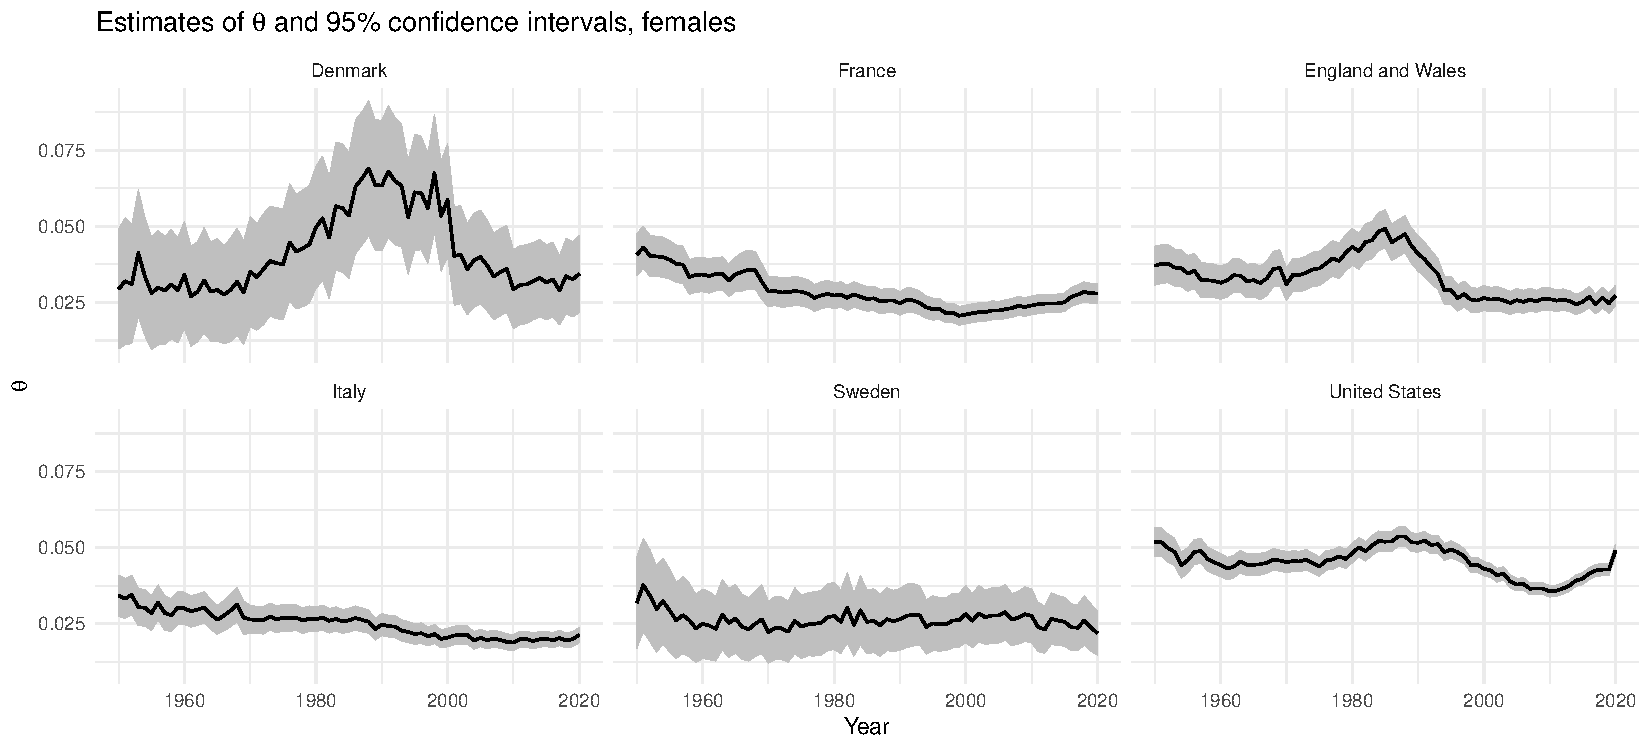
\includegraphics[width=\textwidth]{application/estimates_theta.pdf}
\caption{Estimates of $\theta$ (line) and 95\% Wald confidence intervals (shaded area) for females, 1950--2020.}
\label{fig:est_theta}
\end{figure}

\begin{figure}[htb!]
\centering
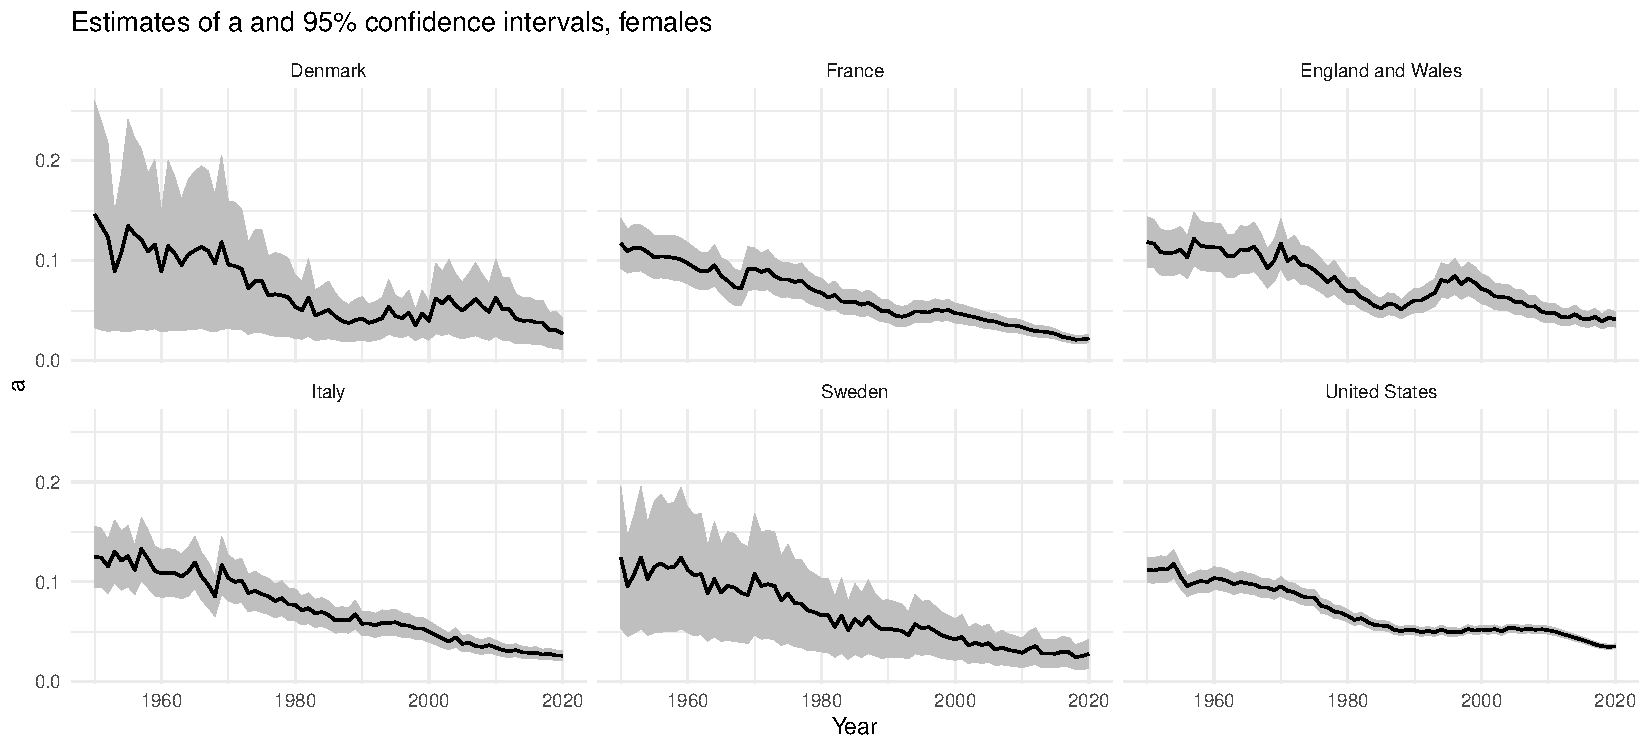
\includegraphics[width=\textwidth]{application/estimates_a.pdf}
\caption{Estimates of $a$ (line) and 95\% Wald confidence intervals (shaded area) for females, 1950--2020.}
\label{fig:est_a}
\end{figure}

\begin{figure}[htb!]
\centering
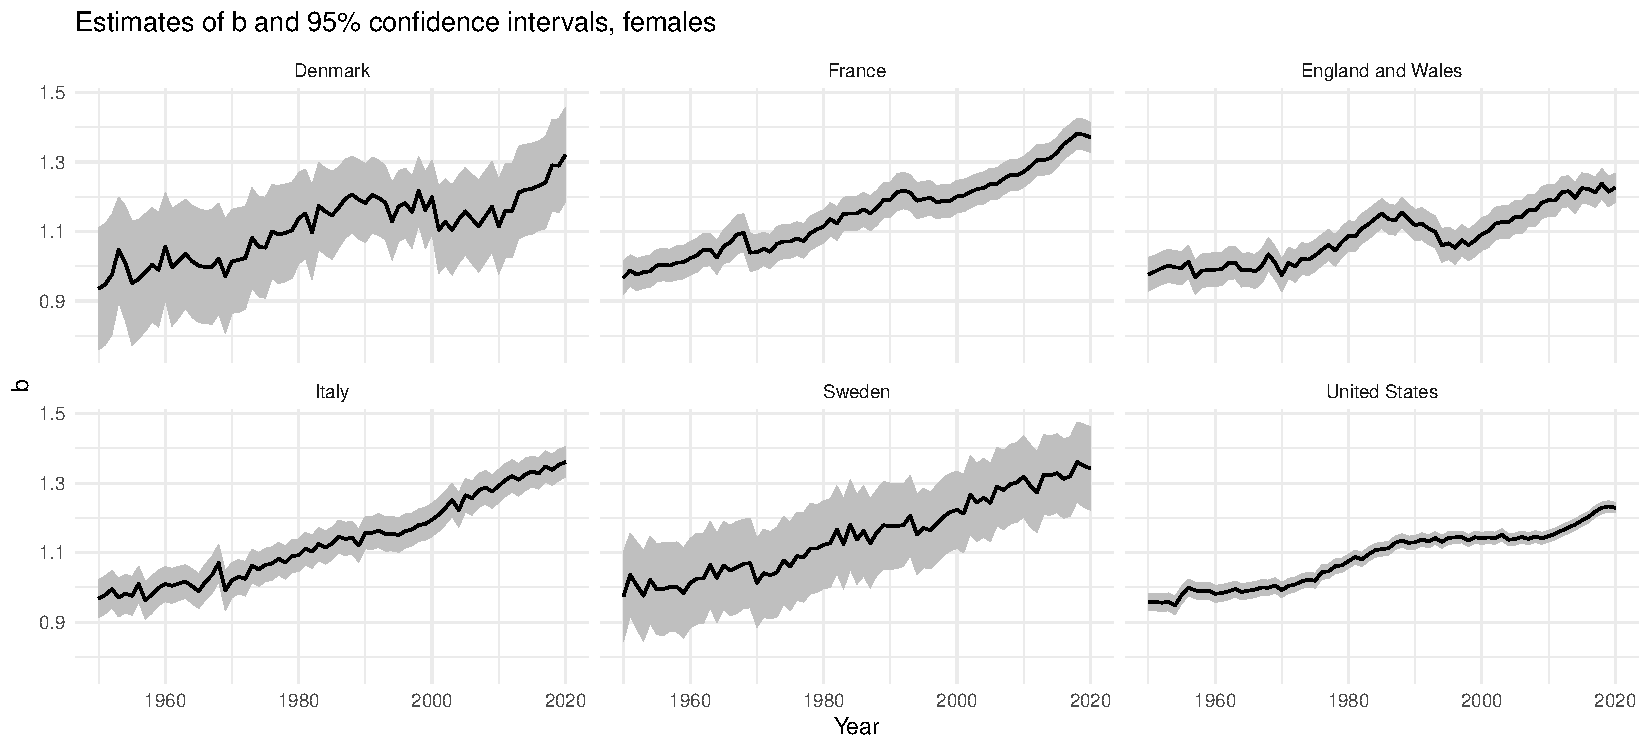
\includegraphics[width=\textwidth]{application/estimates_b.pdf}
\caption{Estimates of $b$ (line) and 95\% Wald confidence intervals (shaded area) for females, 1950--2020.}
\label{fig:est_b}
\end{figure}

\begin{figure}[htb!]
\centering
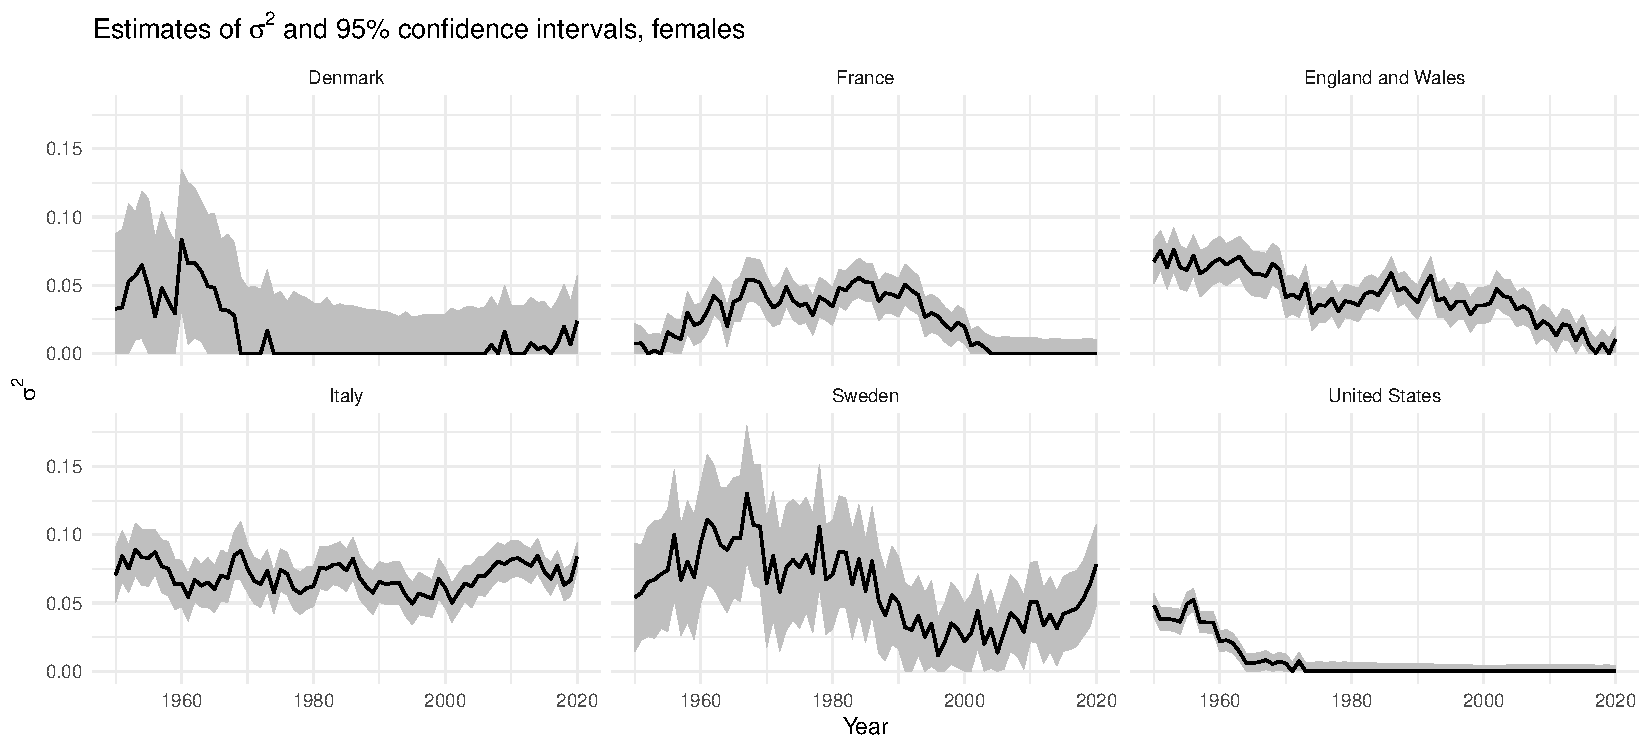
\includegraphics[width=\textwidth]{application/estimates_sigma2.pdf}
\caption{Estimates of $\sigma^2$ (line) and approximate 95\% Wald intervals (shaded area) for females, 1950--2020, with negative lower limits set to zero. The intervals are not valid where $\hat\sigma^2=0$.}
\label{fig:est_sigma2}
\end{figure}

\subsection{Comparison with other mortality laws}

To see whether the extra flexibility of the GLW model improves on established mortality laws, and not only on its gamma-Gompertz submodel, we fit the Gompertz law $\mu(x)=\alpha\e^{\beta x}$ and the Kannisto law $\mu(x)=\alpha\e^{\beta x}/(1+\alpha\e^{\beta x})$ \citep{thatcher1998force} to the same 426 populations, ages and likelihood. Like the GLW and gamma-Gompertz models, both describe senescent mortality only, so we do not include laws with an age-independent Makeham term. For each population we compute $\Delta\mathrm{AIC}_m=\mathrm{AIC}_m-\min_m\mathrm{AIC}_m$ over the four models $m$, and the error of the remaining life expectancy at ages 50, 65 and 80. Since the models are fitted and evaluated on the same population-years, these errors measure their in-sample reproduction of the life-table quantities rather than out-of-sample forecasting performance. Table~\ref{tab:benchmark} summarises the results. In the Appendix, Figure~\ref{fig:bench_daic} shows $\Delta\mathrm{AIC}$ by country and year, Figure~\ref{fig:bench_hazards} the fitted hazards in 2020, and Figures~\ref{fig:bench_ex50} to~\ref{fig:bench_ex80} the errors in the remaining life expectancy.

The GLW model has the lowest AIC in 78\% of the population-years, and its median $\Delta\mathrm{AIC}$ is zero. The advantage is concentrated in recent decades. The GLW model has the lowest AIC in 32\% of the population-years in 1950--1969, when $\hat b$ is close to 1 and the gamma-Gompertz model is preferred in 62\% of them, in 88\% in 1970--1989 and in all population-years from 1990. The ranking does not depend on the penalty for the extra parameter: with BIC instead of AIC, the GLW model is preferred in 73\% of the population-years. The gain in life expectancy is smaller than the gain in likelihood, but it is consistent at older ages. The mean absolute error of $\mathring{e}_{65}$ is 0.145 years for the GLW model, against 0.159 to 0.214 years for the other three laws, and that of $\mathring{e}_{80}$ is 0.088 years, against 0.091 to 0.109 years. At age 50, the Gompertz, gamma-Gompertz and GLW models are equally accurate, with mean absolute errors of about 0.03 years, while the Kannisto law has twice that error. The GLW model does not remove the remaining errors: all four laws underestimate $\mathring{e}_{65}$ in recent years (Figure~\ref{fig:bench_ex65}).

\begin{table}[tbp]
\centering
\small
\caption{Comparison of the GLW model with three mortality laws over the 426 population-years (females, ages 50--109, 1950--2020). $\Delta\mathrm{AIC}_m=\mathrm{AIC}_m-\min_m\mathrm{AIC}_m$ within each population-year; Best AIC is the percentage of population-years in which the model has the lowest AIC; MAE is the mean absolute error, in years, of the estimated remaining life expectancy.}
\label{tab:benchmark}
\begin{tabular*}{\textwidth}{@{\extracolsep{\fill}}lrrrrrr}
\toprule
Model & Parameters & Median $\Delta\mathrm{AIC}$ & Best AIC (\%) & MAE $\mathring{e}_{50}$ & MAE $\mathring{e}_{65}$ & MAE $\mathring{e}_{80}$\\
\midrule
GLW & 4 & 0.0 & 77.7 & 0.031 & 0.145 & 0.088\\
Gamma-Gompertz & 3 & 33.1 & 19.5 & 0.030 & 0.171 & 0.091\\
Kannisto & 2 & 421.3 & 0.7 & 0.067 & 0.214 & 0.109\\
Gompertz & 2 & 112.0 & 2.1 & 0.027 & 0.159 & 0.091\\
\bottomrule
\end{tabular*}
\end{table}

\subsection{Life expectancy, annuities and assurances}

From the GLW estimates we compute the remaining life expectancy $\mathring{e}_x$, the single life annuity $\bar{a}_x$ and the single assurance $\bar{A}_x$ at ages 50, 65 and 80, with force of interest $\delta=0.05$. These ages correspond to $x=0$, 15 and 30 in Section~\ref{sec:actuarial}. Since $\hat b\neq1$, these quantities are evaluated by numerical integration of ${}_tp_x$, as described in Section~\ref{sec:actuarial}.

Figure~\ref{fig:ex_diff} compares the estimated $\mathring{e}_x$ with the values in the life tables of the Human Mortality Database. At age 50, the difference lies between $-0.07$ and $0.15$ years, or between $-0.2\%$ and $0.5\%$. At age 65, the model underestimates $\mathring{e}_{65}$, and the gap widens over time, reaching $-0.48$ years ($-2.1\%$) in recent years. At age 80, the model overestimates $\mathring{e}_{80}$ by at most 0.19 years ($2.6\%$), and the difference is smaller after 1990. The estimated annuities and assurances for every tenth year from 1950 to 2020 are given in Table~\ref{tab:actuarial} in the Appendix.

\begin{figure}[htb!]
\centering
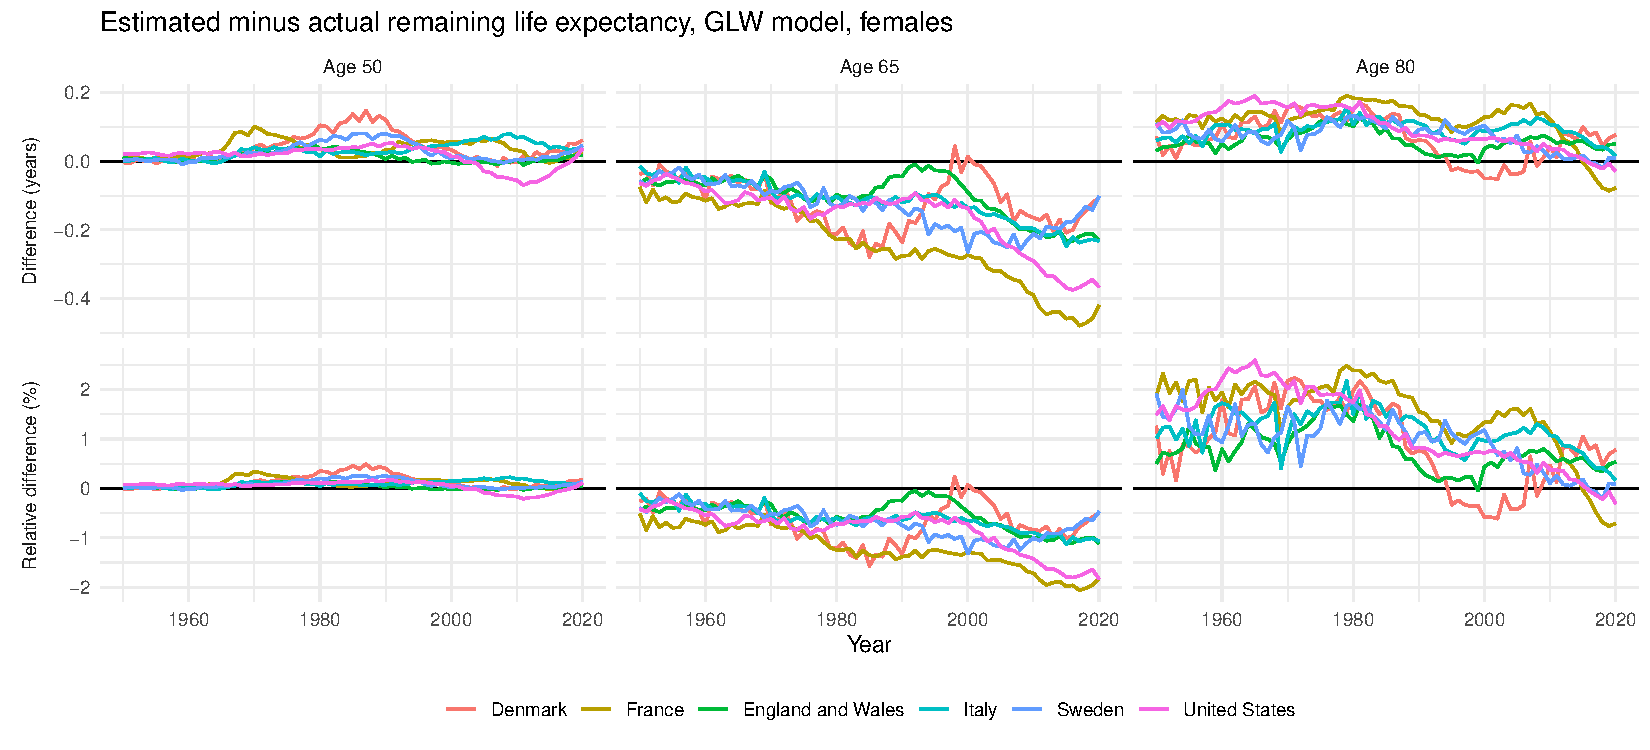
\includegraphics[width=\textwidth]{application/life_expectancy_difference.pdf}
\caption{Difference between the estimated and the actual remaining life expectancy at ages 50, 65 and 80 for females, in years (top) and in percent of the actual value (bottom).}
\label{fig:ex_diff}
\end{figure}

\FloatBarrier
%  ------------------------------------------------------------
\section{Concluding remarks}\label{sec:conclusion}
%  ------------------------------------------------------------

Actuarial mortality models need enough flexibility in the shape of the hazard at old ages. In the gamma-Gompertz model with positive frailty variance, the population hazard always levels off at old ages. We studied the GLW model, which adds gamma frailty to the LW distribution, itself the Weibull extension of \citet{xie2002modified}. Its derivation from the generating function of the Laguerre polynomials gives a series representation in terms of distributions of maxima, and, for positive frailty variance, a single shape parameter, $b$, determines whether the population hazard grows without bound, levels off or declines at old ages.

The survival and hazard functions are in closed form, and the moments, the generating functions, the Shannon entropy and the Kullback--Leibler divergence have explicit representations in terms of special functions and series. At every age $x$, $a(x+T_x)^b-ax^b$ has the distribution of $aX^b$ with an age-dependent $\theta_x$, so the future lifetime stays in the gamma-Gompertz family when $b=1$. The joint-life status of two lives of the same age is again a GLW model when $\sigma_1^2\theta_1=\sigma_2^2\theta_2$. Life annuities and assurances are explicit at every age when $b=1$ and at the starting age when $b>1$, and one-dimensional integrals otherwise. In the simulation study, the Poisson maximum likelihood estimators have small bias and the likelihood-ratio test of $H_0\colon b=1$ keeps its nominal level. The Wald intervals exhibit undercoverage at the cohort sizes considered, although coverage improves as the cohort grows.

In the application to female mortality after age 50, $\hat b$ increased from just below 1 in 1950 to between 1.23 and 1.37 in 2020 in all six countries, and the gamma-Gompertz model is rejected in every year from 1990, also when the test is calibrated by the bootstrap. The GLW model does not dominate the established laws everywhere. In the 1950s and 1960s, when $\hat b$ is close to 1, the gamma-Gompertz model is usually preferred, and at age 50 the Gompertz law reproduces the remaining life expectancy as well as the GLW model. The GLW model is usually preferred from 1970 to 1989 and is preferred in every population-year from 1990, and it gives modest but consistent gains in the accuracy of the remaining life expectancy at ages 65 and 80.

When $\sigma^2>0$, $\bar\mu(x)$ behaves like $ab\,x^{b-1}/\sigma^2$ at older ages, so for $b>1$ the GLW hazard grows polynomially without bound and cannot level off. When $\hat\sigma^2=0$, as in 111 of the fits, the hazard is the LW hazard, which grows faster because of the factor $\e^{ax^b}$. In both cases the hazard implied beyond the range of the data should be used with care, in particular for annuities sold at advanced ages. A Makeham term \citep{makeham1860law} would add background mortality to the model. Its survival factor $\e^{-ct}$ combines with the discount factor, so annuity values would follow from those of Section~\ref{sec:actuarial} at force of interest $\delta+c$; we did not pursue this extension because background mortality is small after age 50 and $c$ would be weakly identified.

Within the data analysed, the additional shape parameter captures a systematic change in old-age mortality that the gamma-Gompertz model cannot represent. The model allows a frailty interpretation and keeps the gamma-Gompertz model as a testable special case and the actuarial quantities in tractable form. The data, however, do not always support heterogeneity: in 111 of the 426 fits the frailty variance is estimated at zero, the fitted model is the homogeneous LW distribution, and the improvement in fit comes from $b$ alone.


%  ------------------------------------------------------------
%  Acknowledgement
%  ------------------------------------------------------------
\section*{Acknowledgement}

\paragraph*{Funding:}
Fredy Castellares was supported by FAPESP (S\~ao Paulo, Brazil) under Grant \textcolor{red}{[grant number]}. Silvio C. Patricio was funded by the European Union (ERC, Born Once -- Die Once, Grant agreement ID 101043983). Views and opinions expressed are those of the authors only and do not necessarily reflect those of the European Union or the European Research Council Executive Agency. Neither the European Union nor the granting authority can be held responsible for them.

\paragraph*{Disclosure statement:}
The authors report there are no competing interests to declare.

\paragraph*{Author contributions (CRediT):}
Software and Visualization: S.C.P.; Conceptualization, Project administration, Supervision and Validation: F.C.; Formal analysis, Investigation, Methodology, Writing -- original draft, review \& editing: F.C. and S.C.P.

\paragraph*{Data and code availability.}
The {\sf R} code that reproduces the simulation study, the application, all figures and all tables is available at 
\begin{center}
    \url{https://github.com/scpatricio/laguerre_weibull_distribution}.
\end{center}
The repository also contains the estimates and model comparisons for all 426 population-years. The mortality data were obtained from the Human Mortality Database \citep{hmd}.

\paragraph*{Declaration of generative AI use:}
During the preparation of this work, the authors used Claude Opus 5.5 (Anthropic) for English language editing and proofreading. The authors reviewed and edited all output, and take full responsibility for the final text.

%  ------------------------------------------------------------
%  References
%  ------------------------------------------------------------
\bibliographystyle{apalike}
\bibliography{references}

%  ------------------------------------------------------------
%  Appendices
%  ------------------------------------------------------------

\clearpage

%%%%%%%%%%%%%%%% START OF SUPPLEMENT %%%%%%%%%%%%%%%

% Figures, tables, equations and pages in the supplement are numbered S1, S2 etc.

\renewcommand{\thefigure}{S\arabic{figure}}
\renewcommand{\thetable}{S\arabic{table}}
\renewcommand{\theequation}{S\arabic{equation}}
\renewcommand{\thepage}{S\arabic{page}}
\setcounter{figure}{0}
\setcounter{table}{0}
\setcounter{equation}{0}
\setcounter{page}{1} % not 0 as \newpage already started a supplementary page

\appendix
\section*{Appendix}

\subsection*{Single life annuity and assurance}

Table~\ref{tab:actuarial} gives the estimated single life annuity and single assurance at ages 50, 65 and 80 for females every 10 years from 1950 to 2020.

\begin{table}[htb!]
\centering
\footnotesize
\renewcommand{\arraystretch}{0.7}
\caption{Estimated single life annuity $\bar{a}_x$ and single assurance $\bar{A}_x$ at ages $x=50$, 65 and 80 for females, with force of interest $\delta=0.05$.}
\label{tab:actuarial}
\begin{tabular*}{\textwidth}{@{\extracolsep{\fill}}llrrrrrr}
\toprule
& & \multicolumn{3}{c}{Single life annuity} & \multicolumn{3}{c}{Single assurance}\\
\cmidrule(lr){3-5}\cmidrule(lr){6-8}
Country & Year & $\bar{a}_{50}$ & $\bar{a}_{65}$ & $\bar{a}_{80}$ & $\bar{A}_{50}$ & $\bar{A}_{65}$ & $\bar{A}_{80}$\\
\midrule
Denmark & 1950 & 13.8655 & 9.4079 & 4.6770 & 0.3067 & 0.5296 & 0.7662\\
 & 1960 & 14.2597 & 9.8646 & 4.9753 & 0.2870 & 0.5068 & 0.7512\\
 & 1970 & 14.5409 & 10.4698 & 5.7079 & 0.2730 & 0.4765 & 0.7146\\
 & 1980 & 14.7751 & 10.8343 & 6.0740 & 0.2612 & 0.4583 & 0.6963\\
 & 1990 & 14.7713 & 10.9085 & 6.2565 & 0.2614 & 0.4546 & 0.6872\\
 & 2000 & 14.9743 & 11.1704 & 6.4828 & 0.2513 & 0.4415 & 0.6759\\
 & 2010 & 15.4156 & 11.6785 & 6.8140 & 0.2292 & 0.4161 & 0.6593\\
 & 2020 & 15.8787 & 12.2941 & 7.3065 & 0.2061 & 0.3853 & 0.6347\\
\addlinespace[3pt]
England and Wales & 1950 & 13.8878 & 9.5287 & 4.9103 & 0.3056 & 0.5236 & 0.7545\\
 & 1960 & 14.2685 & 10.0017 & 5.2669 & 0.2866 & 0.4999 & 0.7367\\
 & 1970 & 14.4094 & 10.2707 & 5.5731 & 0.2795 & 0.4865 & 0.7213\\
 & 1980 & 14.6322 & 10.6123 & 5.8821 & 0.2684 & 0.4694 & 0.7059\\
 & 1990 & 14.9504 & 11.0620 & 6.3113 & 0.2525 & 0.4469 & 0.6844\\
 & 2000 & 15.3140 & 11.4816 & 6.5752 & 0.2343 & 0.4259 & 0.6712\\
 & 2010 & 15.7499 & 12.1036 & 7.1291 & 0.2125 & 0.3948 & 0.6435\\
 & 2020 & 15.7581 & 12.0834 & 7.0334 & 0.2121 & 0.3958 & 0.6483\\
\addlinespace[3pt]
France & 1950 & 13.8884 & 9.6170 & 4.9955 & 0.3056 & 0.5192 & 0.7502\\
 & 1960 & 14.3439 & 10.0867 & 5.2379 & 0.2828 & 0.4957 & 0.7381\\
 & 1970 & 14.7240 & 10.5835 & 5.6628 & 0.2638 & 0.4708 & 0.7169\\
 & 1980 & 15.1540 & 11.1620 & 6.1155 & 0.2423 & 0.4419 & 0.6942\\
 & 1990 & 15.6160 & 11.8259 & 6.7193 & 0.2192 & 0.4087 & 0.6640\\
 & 2000 & 15.9186 & 12.3008 & 7.2213 & 0.2041 & 0.3850 & 0.6389\\
 & 2010 & 16.1823 & 12.7680 & 7.8212 & 0.1909 & 0.3616 & 0.6089\\
 & 2020 & 16.2561 & 12.8593 & 7.8639 & 0.1872 & 0.3570 & 0.6068\\
\addlinespace[3pt]
Italy & 1950 & 13.9029 & 9.5115 & 4.8641 & 0.3049 & 0.5244 & 0.7568\\
 & 1960 & 14.2488 & 9.8712 & 5.0068 & 0.2876 & 0.5064 & 0.7497\\
 & 1970 & 14.5563 & 10.2854 & 5.3606 & 0.2722 & 0.4857 & 0.7320\\
 & 1980 & 14.9167 & 10.7627 & 5.6901 & 0.2542 & 0.4619 & 0.7155\\
 & 1990 & 15.3985 & 11.4799 & 6.3690 & 0.2301 & 0.4260 & 0.6816\\
 & 2000 & 15.8045 & 12.0857 & 6.9485 & 0.2098 & 0.3957 & 0.6526\\
 & 2010 & 16.1551 & 12.6033 & 7.4212 & 0.1922 & 0.3698 & 0.6289\\
 & 2020 & 16.1282 & 12.5263 & 7.2498 & 0.1936 & 0.3737 & 0.6375\\
\addlinespace[3pt]
Sweden & 1950 & 13.9537 & 9.5082 & 4.7497 & 0.3023 & 0.5246 & 0.7625\\
 & 1960 & 14.3930 & 9.9852 & 5.0348 & 0.2803 & 0.5007 & 0.7483\\
 & 1970 & 14.8351 & 10.6814 & 5.7122 & 0.2582 & 0.4659 & 0.7144\\
 & 1980 & 15.1148 & 11.0886 & 6.0522 & 0.2443 & 0.4456 & 0.6974\\
 & 1990 & 15.4217 & 11.5266 & 6.4169 & 0.2289 & 0.4237 & 0.6792\\
 & 2000 & 15.6356 & 11.8766 & 6.7879 & 0.2182 & 0.4062 & 0.6606\\
 & 2010 & 15.9136 & 12.2632 & 7.1193 & 0.2043 & 0.3868 & 0.6440\\
 & 2020 & 16.0957 & 12.4934 & 7.2574 & 0.1952 & 0.3753 & 0.6371\\
\addlinespace[3pt]
United States & 1950 & 13.8102 & 9.7717 & 5.4818 & 0.3095 & 0.5114 & 0.7259\\
 & 1960 & 14.1936 & 10.1731 & 5.6863 & 0.2903 & 0.4913 & 0.7157\\
 & 1970 & 14.4224 & 10.5442 & 6.0887 & 0.2789 & 0.4728 & 0.6956\\
 & 1980 & 14.8559 & 11.1093 & 6.5812 & 0.2572 & 0.4445 & 0.6709\\
 & 1990 & 15.0690 & 11.4020 & 6.8637 & 0.2466 & 0.4299 & 0.6568\\
 & 2000 & 15.1771 & 11.4395 & 6.7291 & 0.2411 & 0.4280 & 0.6635\\
 & 2010 & 15.4977 & 11.8842 & 7.1582 & 0.2251 & 0.4058 & 0.6421\\
 & 2020 & 15.3805 & 11.7139 & 6.9753 & 0.2310 & 0.4143 & 0.6512\\
\bottomrule
\end{tabular*}
\end{table}

\clearpage
\subsection*{Life expectancy errors of the four mortality laws}

Figures~\ref{fig:bench_ex50} to~\ref{fig:bench_ex80} show the difference between the estimated and the actual remaining life expectancy at ages 50, 65 and 80 for the four mortality laws of Section~\ref{sec:application}, in years and in percent of the actual value.

\begin{figure}[htb!]
\centering
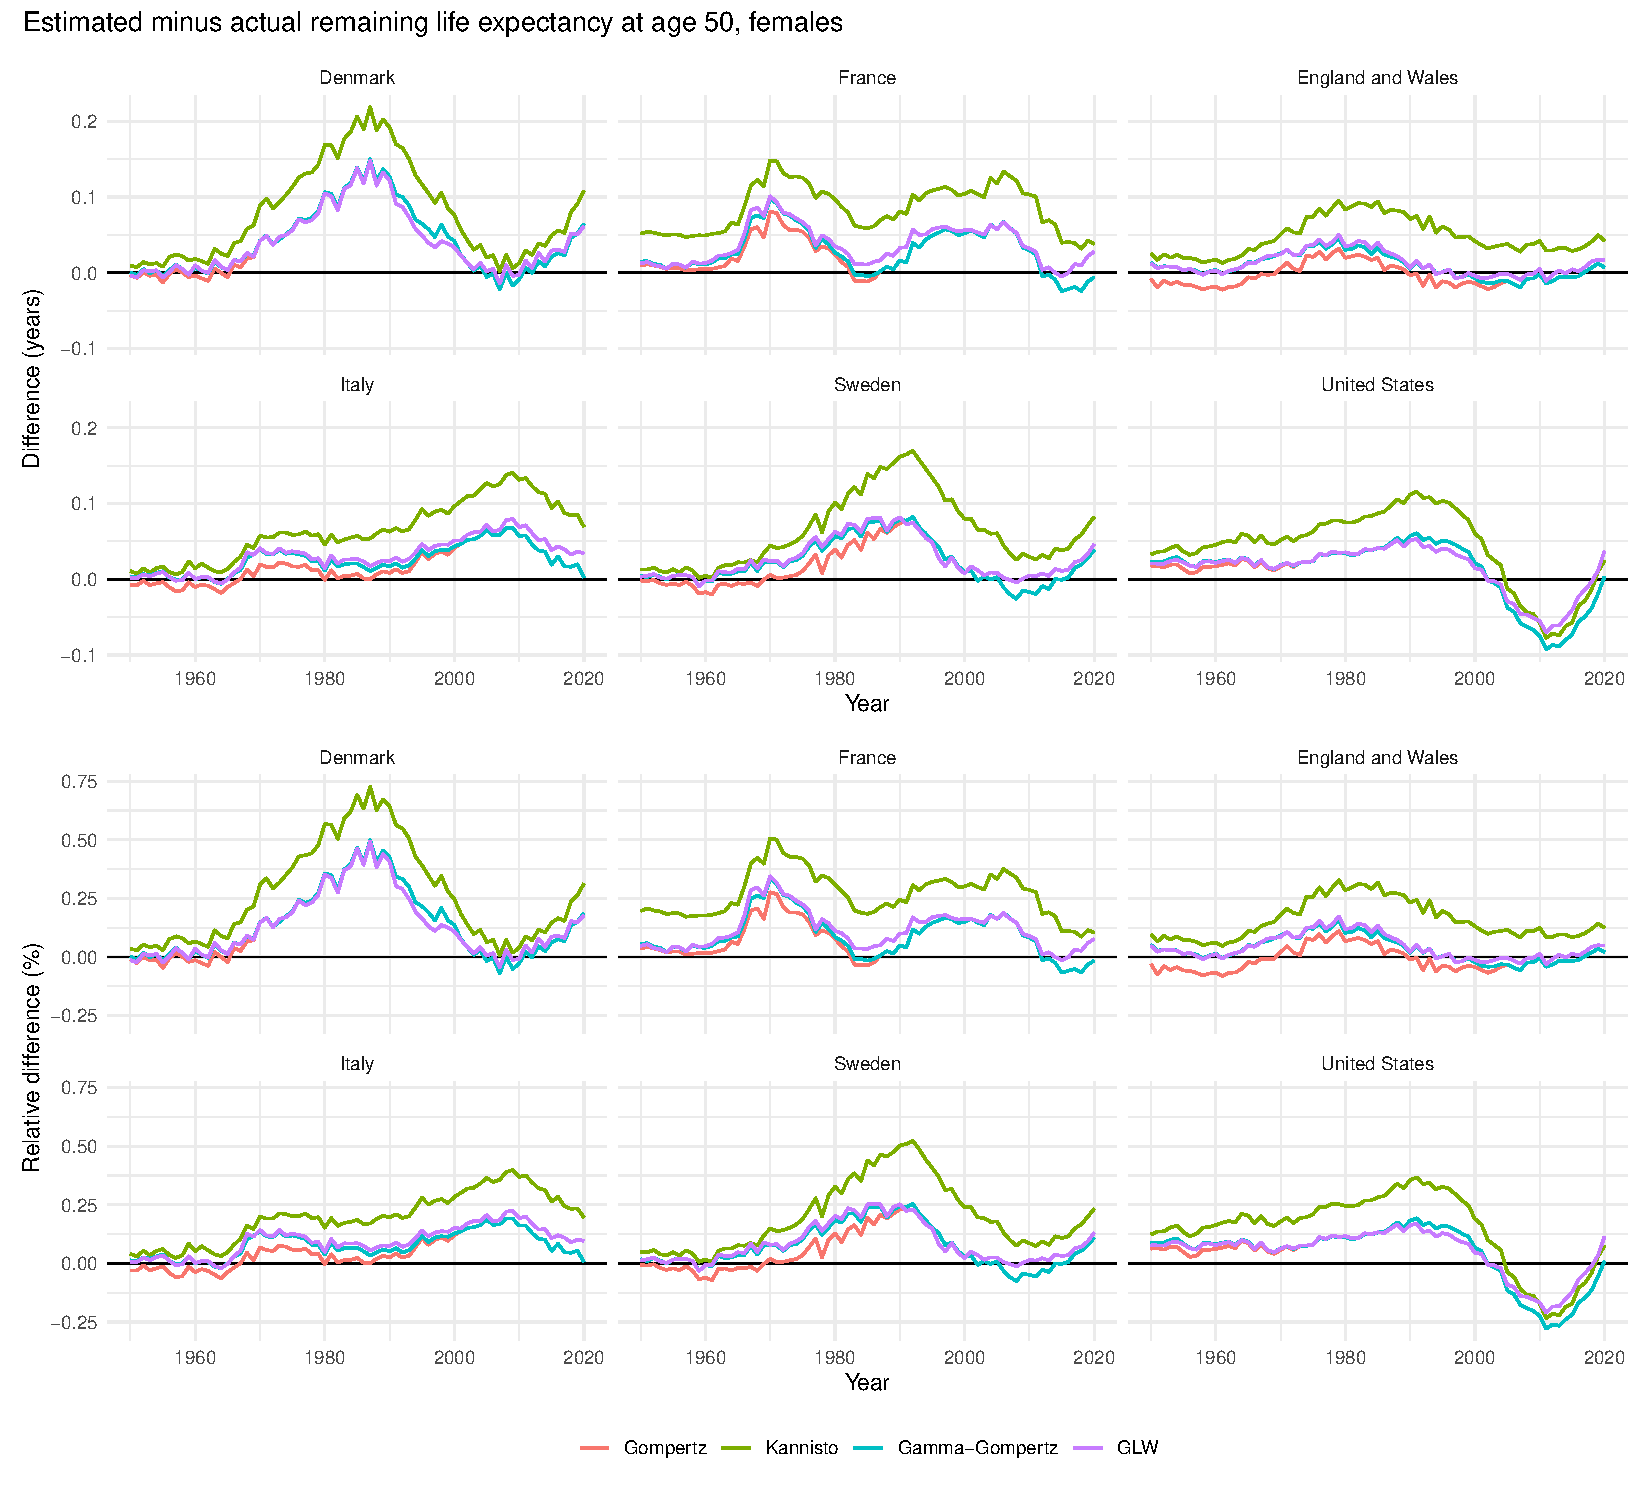
\includegraphics[width=\textwidth]{application/benchmark_ex50.pdf}
\caption{Estimated minus actual remaining life expectancy at age 50 for females, by country, for the four mortality laws, in years (top six panels) and in percent of the actual value (bottom six panels).}
\label{fig:bench_ex50}
\end{figure}

\begin{figure}[htb!]
\centering
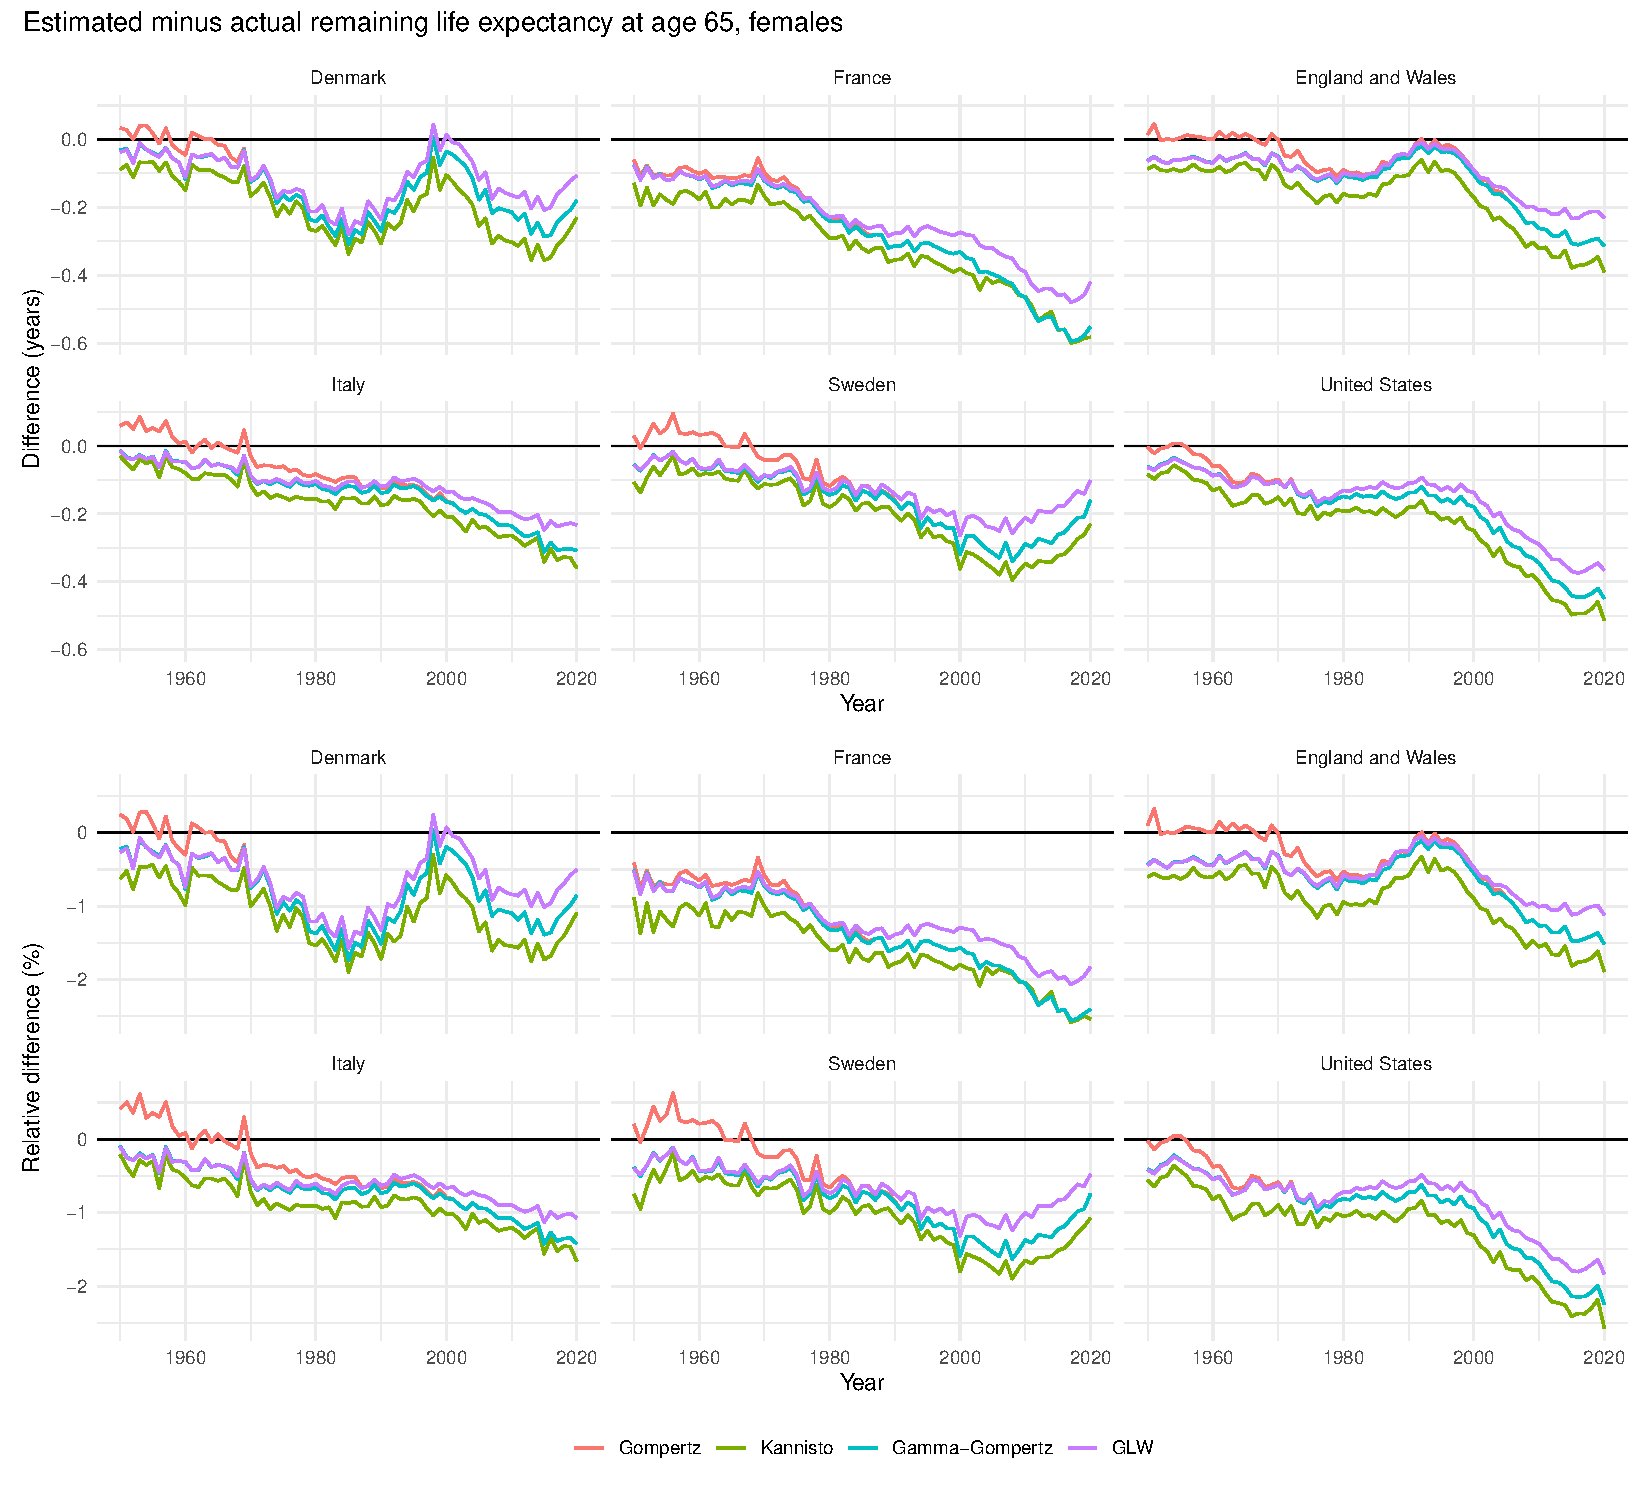
\includegraphics[width=\textwidth]{application/benchmark_ex65.pdf}
\caption{Estimated minus actual remaining life expectancy at age 65 for females, by country, for the four mortality laws, in years (top six panels) and in percent of the actual value (bottom six panels).}
\label{fig:bench_ex65}
\end{figure}

\begin{figure}[htb!]
\centering
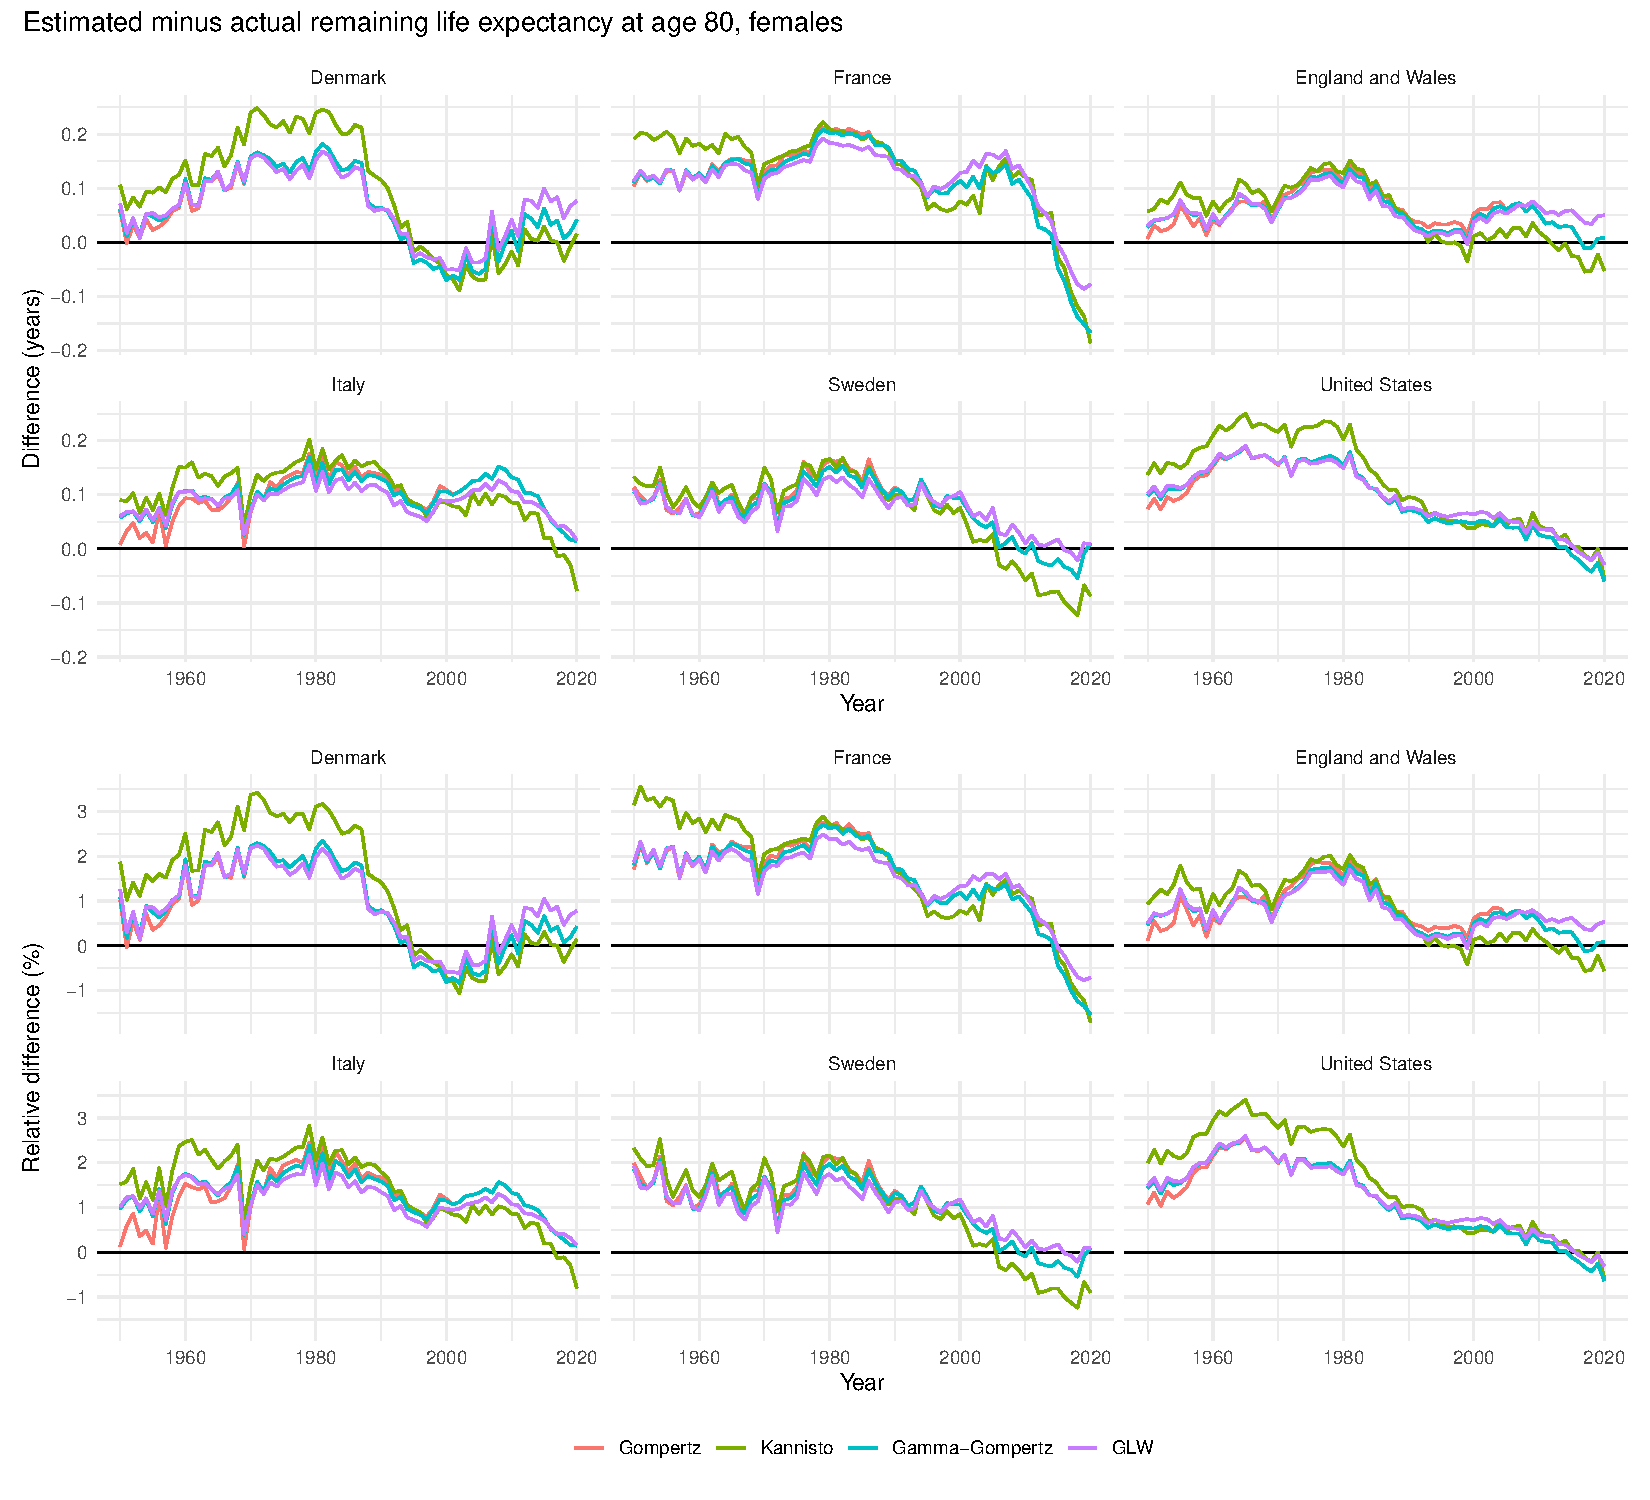
\includegraphics[width=\textwidth]{application/benchmark_ex80.pdf}
\caption{Estimated minus actual remaining life expectancy at age 80 for females, by country, for the four mortality laws, in years (top six panels) and in percent of the actual value (bottom six panels).}
\label{fig:bench_ex80}
\end{figure}

\clearpage
\subsection*{Model fit over time and fitted hazards}

Figure~\ref{fig:bench_daic} shows $\Delta\mathrm{AIC}$ for the four mortality laws of Section~\ref{sec:application} by country and year, and Figure~\ref{fig:bench_hazards} shows the observed and fitted hazards in 2020.

\begin{figure}[htb!]
\centering
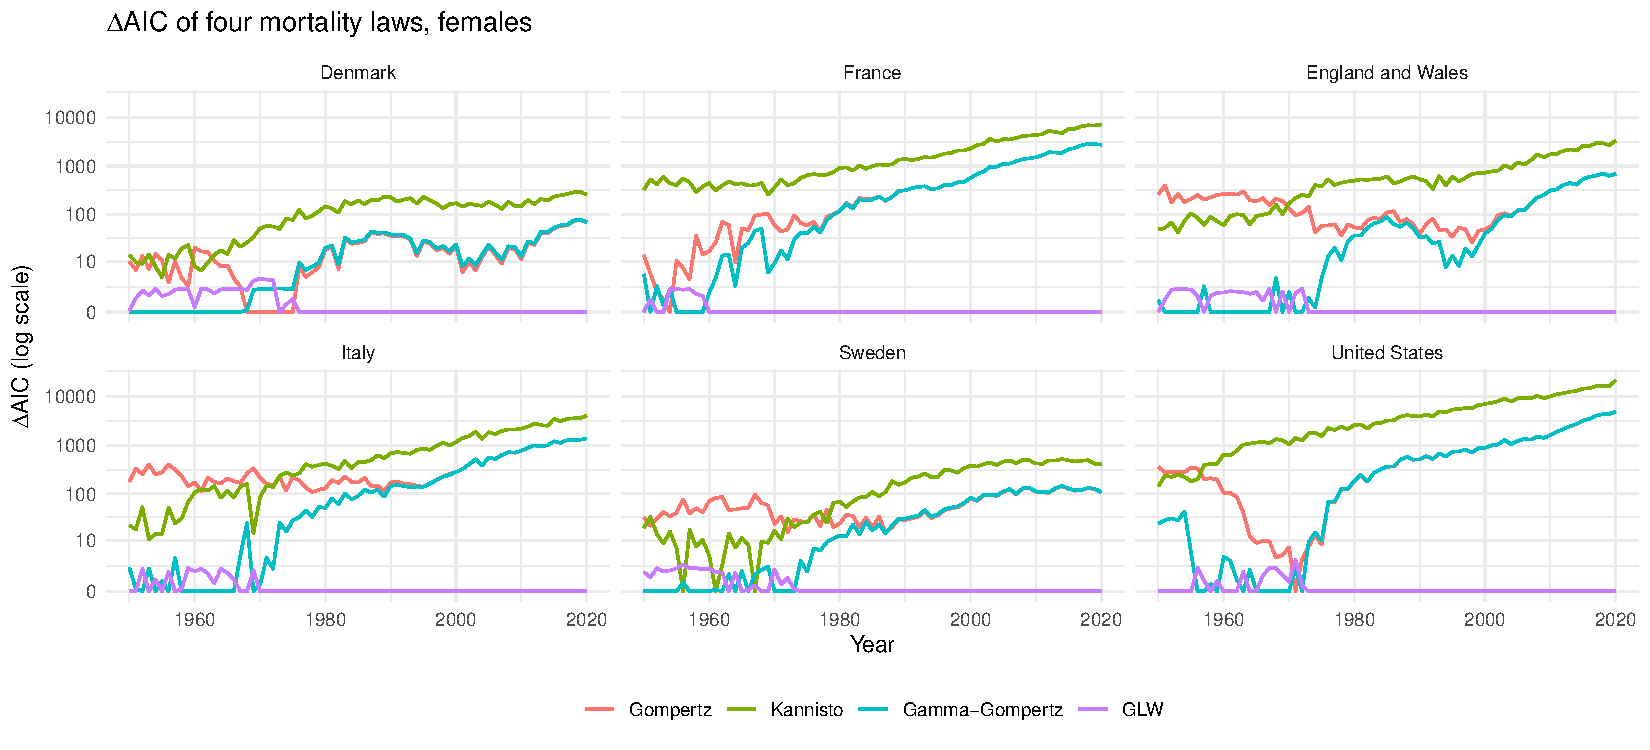
\includegraphics[width=\textwidth]{application/benchmark_daic.pdf}
\caption{$\Delta\mathrm{AIC}_m=\mathrm{AIC}_m-\min_m\mathrm{AIC}_m$ for the four mortality laws, females, by country and year, on a $\log(1+x)$ scale.}
\label{fig:bench_daic}
\end{figure}

\begin{figure}[htb!]
\centering
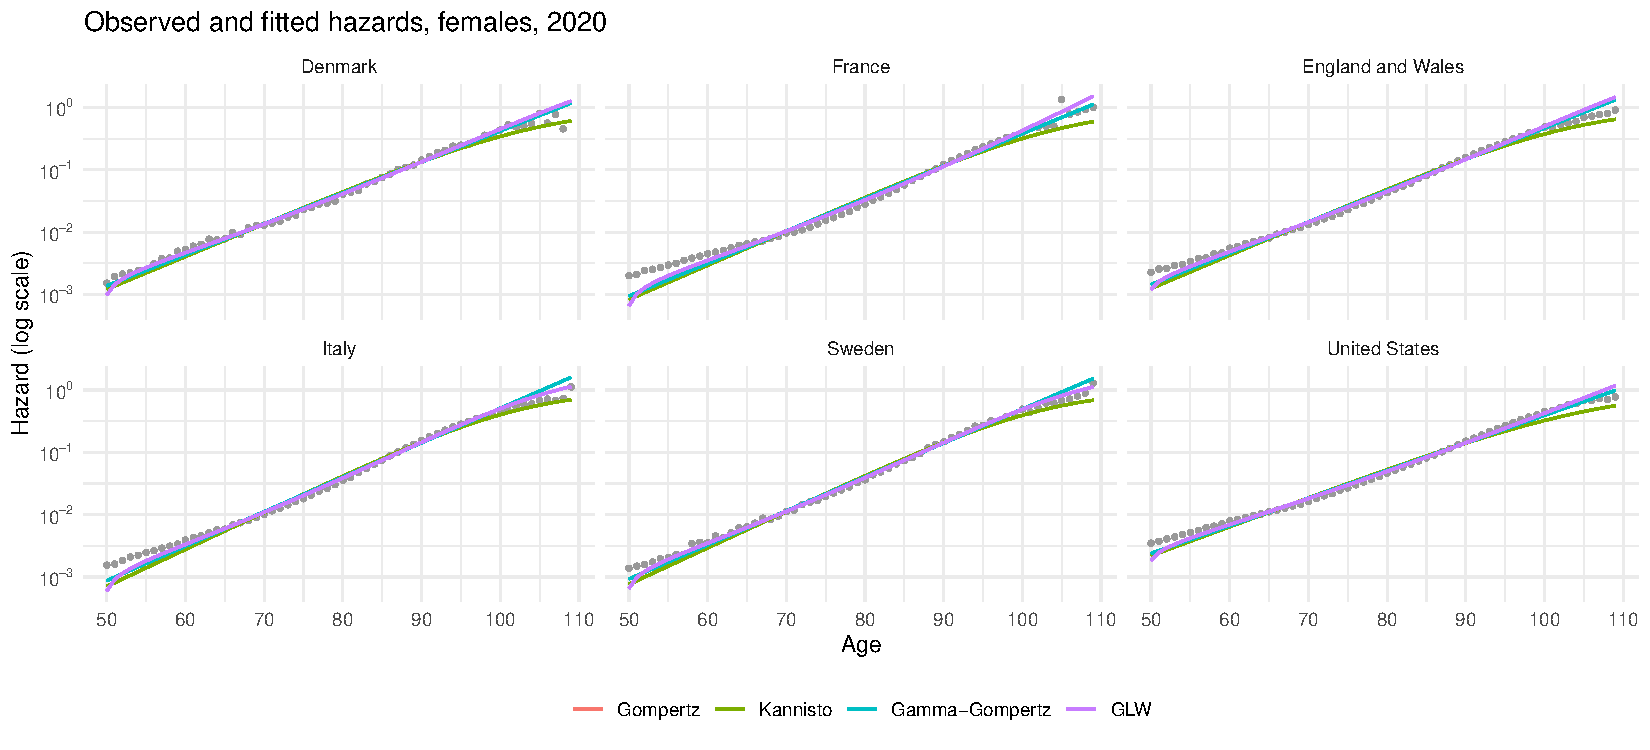
\includegraphics[width=\textwidth]{application/benchmark_hazards.pdf}
\caption{Observed (points) and fitted (lines) hazards for females in 2020, by country, for the four mortality laws, on a log scale.}
\label{fig:bench_hazards}
\end{figure}

\end{document}
